% =============================================================================
%  OTC-X  ·  Liquidity Intelligence Radar
%  ---------------------------------------------------------------------------
%  Investoren-Katalog  ·  Requirements Engineering nach IREB
%  Technischer Implementierungsleitfaden  ·  Quantitative Methodik
%  ---------------------------------------------------------------------------
%  Autor:   Mihael Atanasov
%  Version: 1.0  ·  Maerz 2026
%  Status:  Freigegeben
% =============================================================================

\documentclass[12pt, a4paper, oneside]{report}

% -- Encoding & Language -------------------------------------------------------
\usepackage[utf8]{inputenc}
\usepackage[T1]{fontenc}
\usepackage[ngerman]{babel}

% -- Typography ----------------------------------------------------------------
\usepackage{lmodern}
\usepackage{microtype}
\usepackage{setspace}
\onehalfspacing
\usepackage{parskip}

% -- Page Geometry & Headers ---------------------------------------------------
\usepackage[
  top=2.8cm, bottom=2.8cm, left=2.5cm, right=2.5cm,
  headheight=14pt
]{geometry}
\usepackage{fancyhdr}
\pagestyle{fancy}
\fancyhf{}
\renewcommand{\headrulewidth}{0.4pt}
\renewcommand{\footrulewidth}{0.2pt}
\fancyhead[L]{\small\textcolor{swissred}{\textbf{OTC-X}} \textcolor{darknavy}{\,\textbullet\, Liquidity Intelligence Radar}}
\fancyhead[R]{\small\textcolor{darknavy}{\nouppercase{\leftmark}}}
\fancyfoot[C]{\small\textcolor{darknavy}{\thepage}}
\fancyfoot[R]{\tiny\textcolor{gray}{v1.0 \,\textbullet\, M\"arz 2026}}

% -- Colours -------------------------------------------------------------------
\usepackage[dvipsnames,svgnames,x11names]{xcolor}
\definecolor{swissred}{HTML}{B22222}
\definecolor{darknavy}{HTML}{1A1A2E}
\definecolor{softgray}{HTML}{F5F6F8}
\definecolor{accentgreen}{HTML}{28A745}
\definecolor{deepcrimson}{HTML}{7D1128}
\definecolor{codebg}{HTML}{F8F8F2}
\definecolor{linkblue}{HTML}{2E86AB}
\definecolor{metricblue}{HTML}{2B6CB0}
\definecolor{warnamber}{HTML}{D69E2E}
\definecolor{criticalorange}{HTML}{DD6B20}

% -- Mathematics ---------------------------------------------------------------
\usepackage{amsmath, amssymb, amsthm, mathtools}
\usepackage{bm}

% -- Graphics & Tables ---------------------------------------------------------
\usepackage{graphicx}
\usepackage{booktabs}
\usepackage{tabularx}
\usepackage{longtable}
\usepackage{colortbl}
\usepackage{multirow}
\usepackage{array}
\usepackage{float}
\usepackage{caption}
\captionsetup{
  font={small,sf},
  labelfont={bf,color=swissred},
  format=hang,
  margin=1cm,
}

% -- TikZ for diagrams ---------------------------------------------------------
\usepackage{tikz}
\usetikzlibrary{arrows.meta,positioning,shapes.geometric,calc}

% -- Boxes & Environments ------------------------------------------------------
\usepackage[most]{tcolorbox}
\tcbset{
  sharp corners,
  boxrule=0pt,
  left=8pt, right=8pt, top=6pt, bottom=6pt,
  fonttitle=\sffamily\bfseries,
}

\newtcolorbox{reqbox}[1][]{
  colback=softgray,
  colframe=swissred,
  borderline west={3pt}{0pt}{swissred},
  title={#1},
  coltitle=white,
  colbacktitle=swissred,
  fonttitle=\sffamily\bfseries\small,
}

\newtcolorbox{infobox}[1][]{
  colback=blue!3,
  colframe=linkblue,
  borderline west={3pt}{0pt}{linkblue},
  title={#1},
  coltitle=white,
  colbacktitle=linkblue,
  fonttitle=\sffamily\bfseries\small,
}

\newtcolorbox{mathbox}[1][]{
  colback=softgray,
  colframe=darknavy,
  borderline west={3pt}{0pt}{darknavy},
  title={#1},
  coltitle=white,
  colbacktitle=darknavy,
  fonttitle=\sffamily\bfseries\small,
}

\newtcolorbox{warnbox}[1][]{
  colback=red!3,
  colframe=deepcrimson,
  borderline west={3pt}{0pt}{deepcrimson},
  title={#1},
  coltitle=white,
  colbacktitle=deepcrimson,
  fonttitle=\sffamily\bfseries\small,
}

\newtcolorbox{insightbox}[1][]{
  colback=accentgreen!5,
  colframe=accentgreen!70!black,
  boxrule=0.5pt,
  arc=2mm,
  left=6pt, right=6pt, top=4pt, bottom=4pt,
  fontupper=\itshape,
  #1
}

\newtcolorbox{usecasebox}[1][]{
  colback=metricblue!5,
  colframe=metricblue,
  borderline west={3pt}{0pt}{metricblue},
  title={#1},
  coltitle=white,
  colbacktitle=metricblue,
  fonttitle=\sffamily\bfseries\small,
}

% -- Listings ------------------------------------------------------------------
\usepackage{listings}
\lstset{
  basicstyle=\ttfamily\small,
  backgroundcolor=\color{codebg},
  frame=single,
  rulecolor=\color{gray!40},
  keywordstyle=\color{swissred}\bfseries,
  commentstyle=\color{gray}\itshape,
  stringstyle=\color{accentgreen},
  breaklines=true,
  numbers=left,
  numberstyle=\tiny\color{gray},
  tabsize=4,
  showstringspaces=false,
}

% -- Hyperlinks ----------------------------------------------------------------
\usepackage[
  colorlinks=true,
  linkcolor=swissred,
  urlcolor=linkblue,
  citecolor=darknavy,
  bookmarks=true,
  bookmarksopen=true,
]{hyperref}

% -- Lists ---------------------------------------------------------------------
\usepackage{enumitem}
\setlist[itemize]{leftmargin=1.5em, itemsep=2pt}
\setlist[enumerate]{leftmargin=1.8em, itemsep=2pt}

% -- Section Styling -----------------------------------------------------------
\usepackage{titlesec}
\titleformat{\chapter}[display]
  {\normalfont\huge\bfseries\sffamily\color{darknavy}}
  {\textcolor{swissred}{\rule{4pt}{1.5cm}}\quad\LARGE\textcolor{swissred}{Kapitel \thechapter}}
  {0.5em}
  {}
  [\vspace{-0.5em}{\color{swissred}\rule{\textwidth}{1pt}}]

\titleformat{\section}
  {\normalfont\Large\bfseries\sffamily\color{darknavy}}
  {\textcolor{swissred}{\thesection}}{0.8em}{}

\titleformat{\subsection}
  {\normalfont\large\bfseries\sffamily\color{darknavy}}
  {\textcolor{swissred}{\thesubsection}}{0.7em}{}

\titleformat{\subsubsection}
  {\normalfont\normalsize\bfseries\sffamily\color{darknavy}}
  {\textcolor{swissred}{\thesubsubsection}}{0.6em}{}

% -- Commands ------------------------------------------------------------------
\newcommand{\term}[1]{\textcolor{swissred}{\textsf{\textbf{#1}}}}
\newcommand{\code}[1]{\texttt{\small\textcolor{darknavy}{#1}}}


% =============================================================================
%  DOCUMENT START
% =============================================================================
\begin{document}

% -- TITLE PAGE ----------------------------------------------------------------
\begin{titlepage}
\begin{center}

\vspace*{1.5cm}

{\color{swissred}\rule{\textwidth}{2pt}}
\vspace{0.4cm}

{\fontsize{42}{48}\selectfont\bfseries\sffamily\textcolor{darknavy}{OTC\,|\,X}}

\vspace{0.15cm}
{\Large\sffamily\textcolor{darknavy}{Liquidity Intelligence Radar}}

\vspace{0.3cm}
{\color{swissred}\rule{\textwidth}{2pt}}

\vspace{1.8cm}

\begin{tcolorbox}[
  colback=darknavy,
  colframe=darknavy,
  arc=3mm,
  boxrule=0pt,
  width=0.92\textwidth,
  halign=center,
  top=12pt, bottom=12pt
]
{\fontsize{18}{24}\selectfont\bfseries\color{white}
Investoren-Katalog}\\[6pt]
{\large\color{softgray}
Requirements Engineering nach IREB\;\textbullet\;Technischer Leitfaden\;\textbullet\;Quantitative Methodik}
\end{tcolorbox}

\vspace{2cm}

\begin{tabular}{rl}
  \textcolor{swissred}{\sffamily\textbf{Autor:}}   & \sffamily Mihael Atanasov \\[4pt]
  \textcolor{swissred}{\sffamily\textbf{Auftraggeber:}}  & \sffamily BEKB Trading Desk, Berner Kantonalbank AG \\[4pt]
  \textcolor{swissred}{\sffamily\textbf{Dom\"ane:}} & \sffamily Schweizer OTC-Aktien\,---\,243 ausserb\"orsliche Titel \\[4pt]
  \textcolor{swissred}{\sffamily\textbf{Version:}}  & \sffamily 1.0 \\[4pt]
  \textcolor{swissred}{\sffamily\textbf{Datum:}}    & \sffamily M\"arz 2026 \\[4pt]
  \textcolor{swissred}{\sffamily\textbf{Klassifikation:}} & \sffamily\textcolor{swissred}{\textbf{Propriet\"ar \& Vertraulich}} \\
\end{tabular}

\vfill

{\small\sffamily\textcolor{darknavy}{Mit Pr\"azision entwickelt\;\;$\bullet$\;\;f\"ur den Schweizer OTC-Markt}}

\vspace{0.3cm}
{\color{swissred}\rule{0.5\textwidth}{0.5pt}}

\end{center}
\end{titlepage}

% -- FRONT MATTER --------------------------------------------------------------
\pagenumbering{roman}
\tableofcontents
\clearpage
\listoftables
\clearpage
\listoffigures
\clearpage

\pagenumbering{arabic}
\setcounter{page}{1}


% =============================================================================
%  KAPITEL 1 --- BEWEGGRUENDE UND PROJEKTGENESE
% =============================================================================
\chapter{Beweggr\"unde und Projektgenese}
\label{ch:beweggruende}

\section{Die Opazit\"at des Schweizer OTC-Marktes}

Der ausserb\"orsliche Handel in der Schweiz\,---\,repr\"asentiert durch die \term{OTC-X}-Plattform der Berner Kantonalbank (BEKB)\,---\,stellt ein faszinierendes Paradoxon dar: obgleich rund 243 Titel mit vereinzelter, mitunter betr\"achtlicher Handelsaktivit\"at dort notiert sind, existiert bis dato kein konsolidiertes Instrument, das diese fragmentierten Datenstr\"ome zu einem koh\"arenten Lagebild verdichtet. Die Konsequenz ist eine strukturelle Informationsasymmetrie, die institutionelle Akteure vor substanzielle Herausforderungen stellt.

\begin{infobox}[Problemstellung]
Der Schweizer OTC-Markt zeichnet sich durch \textbf{fragmentierte Datenquellen}, das \textbf{Fehlen standardisierter Liquidit\"atsmetriken} und \textbf{unsichtbare Anomalie-Signale} aus. Traditionelle Handelsplattformen bieten keine aggregierte Sicht auf markt\"ubergreifende Muster.
\end{infobox}

Dieses Projekt\,---\,\textbf{OTC-X Liquidity Intelligence Radar}\,---\,wurde konzipiert, um genau diese L\"ucke zu schliessen. Es transformiert rohe Transaktionsdaten in ein signalreiches, interaktives Dashboard, das dem BEKB Trading Desk als t\"agliches Entscheidungsinstrument dient.

\section{Das Problemfeld im Detail}

Der Schweizer OTC-Markt, administriert \"uber die Berner B\"orse, weist mehrere Charakteristika auf, die konventionelle Analyseans\"atze als unzul\"anglich entlarven:

\begin{enumerate}[label=\textcolor{swissred}{\textbf{\arabic*.}}]
  \item \textbf{Fragmentierung}\;--- Handelsdaten sind \"uber individuelle Wertpapier-Endpunkte verstreut; eine konsolidierte Sicht existiert nicht.
  \item \textbf{Illiquidit\"at}\;--- Zahlreiche Titel handeln lediglich sporadisch; klassische B\"orsenmetriken (VWAP, kontinuierliche Orderb\"ucher) sind nicht anwendbar.
  \item \textbf{Opazit\"at}\;--- Weder \"offentlich zug\"angliche Liquidit\"ats-Scores noch Anomalie-Benachrichtigungen oder historische Baseline-Vergleiche stehen zur Verf\"ugung.
  \item \textbf{Skalierung}\;--- 243 Wertpapiere mit \"uber 20 Jahren Handelshistorie umfassen circa 133\,000 individuelle Trade-Datens\"atze.
  \item \textbf{Heterogenit\"at}\;--- Die Sektoren erstrecken sich von Banken und Versicherungen \"uber Industrie bis hin zu Immobilien, wobei jeder Sektor ein distinktes Liquidit\"atsprofil aufweist.
\end{enumerate}

\section{Pers\"onliche Motivation und Erkenntnisse}

Die Idee zu diesem Projekt entsprang der \"Uberzeugung, dass quantitative Methoden und moderne Softwarearchitektur auch in vermeintlich \glqq klassischen\grqq{} Marktsegmenten disruptives Potenzial entfalten k\"onnen. Der OTC-Markt\,---\,oft als Nische abgetan\,---\,birgt genau jene Datens\"atze, die sich f\"ur algorithmische Analyse eignen: begrenzte Liquidit\"at erzeugt ausgepr\"agte Signale, und geringe Beobachtungsfrequenz erlaubt es, jede Anomalie isoliert zu betrachten.

\textbf{Zentrale Erkenntnisse:}
\begin{itemize}
  \item Die Implementierung einer \textbf{End-to-End-Pipeline}\,---\,vom Web-Scraping \"uber ETL bis zur Visualisierung\,---\,erfordert ein rigoroses Architekturverst\"andnis, das weit \"uber das Schreiben einzelner Skripte hinausgeht.
  \item \textbf{Polars} als DataFrame-Engine hat den analytischen Durchsatz um eine Gr\"ossenordnung gegen\"uber reinem Pandas beschleunigt, insbesondere bei Rolling-Window-Berechnungen \"uber 75\,000+ Zeilen.
  \item Die Konzeption eines \textbf{Anomaly-Scoring-Systems} verlangt nicht nur mathematische Korrektheit, sondern auch dom\"anenspezifische Kalibrierung: Schwellenwerte, die in einem liquiden Markt trivial w\"aren, entfalten im OTC-Segment ihre volle diagnostische Kraft.
\end{itemize}

\section{Vision und Weiterentwicklung}

Die aktuelle Version stellt den Grundstein dar. K\"unftige Iterationen sollen folgende Dimensionen erschliessen:

\begin{enumerate}
  \item \textbf{Pr\"adiktive Analytik}\;--- Integration von ARIMA- und GARCH-Modellen zur Volatilit\"atsprognose.
  \item \textbf{NLP-gest\"utzte Nachrichtenanalyse}\;--- Sentiment-Scoring aus Schweizer Finanzmedien als zus\"atzlicher Anomalie-Trigger.
  \item \textbf{Echtzeit-Streaming}\;--- Migration von Batch-basierter Verarbeitung zu einer eventgetriebenen Architektur (Apache Kafka / Redis Streams).
  \item \textbf{Multi-Mandanten-F\"ahigkeit}\;--- Erweiterung des Dashboards f\"ur weitere Marktplatzbetreiber.
\end{enumerate}

\begin{insightbox}
Die ultimative Ambition besteht darin, OTC-X nicht bloss als retrospektives Analysewerkzeug zu positionieren, sondern als \textbf{vorausschauendes Entscheidungsunterst\"utzungssystem}\,---\,ein W\"achter, der den Schweizer OTC-Markt observiert, damit die H\"andler es nicht m\"ussen.
\end{insightbox}


% =============================================================================
%  KAPITEL 2 --- PROJEKTZIELE UND STRATEGISCHER MEHRWERT
% =============================================================================
\chapter{Projektziele und strategischer Mehrwert}
\label{ch:projektziele}

\section{Projekthintergrund}

Die Berner Kantonalbank (BEKB) betreibt mit der OTC-X-Plattform den gr\"ossten ausserb\"orslichen Handelsplatz der Schweiz. T\"aglich werden dort Transaktionen in rund 243 nichtkotierten Wertpapieren abgewickelt. Dennoch verf\"ugt das Trading Desk bis dato \"uber kein systematisches Instrument zur Liquidit\"atsmessung, Anomalie-Erkennung oder Risikoquantifizierung dieser Titel. Die vorhandenen Daten werden weder konsolidiert noch analytisch aufbereitet\,---\,ein Umstand, der angesichts des kumulierten Handelsvolumens von \"uber CHF 500 Millionen j\"ahrlich als eklatantes Defizit zu bewerten ist.

\section{Strategische Projektziele}

\begin{enumerate}[label=\textcolor{swissred}{\textbf{Z\arabic*.}}]
  \item \textbf{Transparenzgewinn:} Automatisierte, t\"agliche Konsolidierung s\"amtlicher OTC-X-Handelsdaten in ein einheitliches analytisches Dataset.
  \item \textbf{Liquidit\"atsmessung:} Quantitative Erfassung der Illiquidit\"at mittels akademisch fundierter Kennzahlen (Amihud-Ratio, Spread-Proxy, Rolling Baselines).
  \item \textbf{Fr\"uhwarnsystem:} Automatisierte Anomalie-Erkennung \"uber alle 243 Titel mit gewichtetem Severity-Scoring.
  \item \textbf{Entscheidungsunterst\"utzung:} Bereitstellung eines interaktiven Dashboards mit 11 Charttypen f\"ur die t\"agliche Nutzung am Trading Desk.
  \item \textbf{Zeiteffizienz:} Reduktion des Morgenbriefings von 15 Minuten auf 2 Minuten durch konsolidiertes Lagebild.
\end{enumerate}

\section{Wertsch\"opfung: Ohne Radar vs.\ Mit Radar}

Die nachstehende Gegen\"uberstellung verdeutlicht den operativen Paradigmenwechsel, den der \term{Liquidity Intelligence Radar} f\"ur das BEKB Trading Desk bedeutet:

\begin{table}[H]
\centering
\caption{Strategischer Vergleich: Status Quo vs.\ OTC-X Radar}
\label{tab:ohne-mit-radar}
\rowcolors{2}{softgray}{white}
\begin{tabularx}{\textwidth}{>{\bfseries\sffamily}p{3.2cm} X X}
  \toprule
  \rowcolor{darknavy} \textcolor{white}{Dimension} & \textcolor{white}{Ohne Radar} & \textcolor{white}{Mit Radar} \\
  \midrule
  Datenquelle           & Ad-hoc, manuell, fehlerhaft & Systematisch, t\"aglich, verifizierbar \\
  Illiquidit\"at         & \glqq F\"uhlt sich d\"unn an\grqq & Quantifiziert (Amihud + Baseline) \\
  Anomalie-Erkennung    & Zuf\"allig, wenn jemand hinschaut & Automatisiert, t\"aglich, f\"ur alle 243 Titel \\
  Risk-Quantifizierung  & Sch\"atzen & Datengest\"utzt (Spread-Allokation, Severity-Scores) \\
  Timing-Signale        & Keine & Volumen-/Activity-Spikes (Trading-Chancen) \\
  Langfristige Trends   & Keine Sicht & Regime-Wechsel, Sektor-Entwicklung \\
  Kundenberatung        & Generisch & Konkrete, datengest\"utzte Allocation \\
  Operational Speed     & 15\,Min Briefing & 2\,Min Briefing \\
  \bottomrule
\end{tabularx}
\end{table}

\begin{warnbox}[Kernaussage f\"ur Investoren]
Der \term{Liquidity Intelligence Radar} transformiert den Informationszugang des Trading Desk von einer reaktiven, manuellen Praxis hin zu einer proaktiven, datengest\"utzten Entscheidungsinfrastruktur. Die Reduktion der Briefing-Dauer um \textbf{87\,\%} (von 15 auf 2 Minuten) ist dabei nur der sichtbarste Ausdruck eines fundamentalen Effizienzgewinns.
\end{warnbox}

\section{Return on Investment}

Der wirtschaftliche Nutzen des Radars manifestiert sich in drei Dimensionen:

\begin{itemize}
  \item \textbf{Zeitersparnis:} 13 Minuten pro Tag $\times$ 250 Handelstage $=$ \textbf{54 Stunden/Jahr} pro H\"andler, die f\"ur wertsch\"opfende T\"atigkeiten frei werden.
  \item \textbf{Risikominderung:} Fr\"uhzeitige Erkennung von Anomalien reduziert das Exposure gegen\"uber illiquiden Positionen und potenziellen Compliance-Verst\"ossen.
  \item \textbf{Informationsvorsprung:} Automatisierte, t\"agliche Analyse aller 243 Titel schafft einen systematischen Vorteil gegen\"uber manuell operierenden Marktteilnehmern.
\end{itemize}


% =============================================================================
%  KAPITEL 3 --- ANFORDERUNGSKATALOG NACH IREB
% =============================================================================
\chapter{Anforderungskatalog nach IREB}
\label{ch:requirements}

\section{Grundlagen und Methodik}

Das Requirements Engineering f\"ur \term{OTC-X} folgt dem \textbf{IREB CPRE Foundation Level}-Standard (International Requirements Engineering Board, Syllabus v3.1). Die nachstehenden Anforderungskategorien orientieren sich an den vier Kernaktivit\"aten:

\begin{enumerate}[label=\textcolor{swissred}{\textbf{\arabic*.}}]
  \item \textbf{Ermittlung} (Elicitation)\;--- Stakeholder-Interviews, Dokumentenanalyse, API-Exploration
  \item \textbf{Dokumentation} (Documentation)\;--- Strukturierte Spezifikation mit eindeutigen IDs
  \item \textbf{Validierung} (Validation \& Negotiation)\;--- Review-Zyklen mit dem BEKB Trading Desk
  \item \textbf{Verwaltung} (Management)\;--- Versionskontrolle via Git, Traceability durch Modulzuordnung
\end{enumerate}

\section{Stakeholder-Analyse}

\begin{table}[H]
\centering
\caption{Stakeholder-Matrix nach Einfluss und Interesse}
\label{tab:stakeholders}
\rowcolors{2}{softgray}{white}
\begin{tabularx}{\textwidth}{>{\bfseries\sffamily}l X l l}
  \toprule
  \rowcolor{darknavy} \textcolor{white}{Stakeholder} & \textcolor{white}{Rolle \& Interesse} & \textcolor{white}{Einfluss} & \textcolor{white}{Priorit\"at} \\
  \midrule
  BEKB Trading Desk     & Prim\"arer Endnutzer; ben\"otigt t\"agliche Liquidit\"ats\"ubersicht und Anomalie-Alerts & Hoch  & Kritisch \\
  Compliance-Abteilung  & Sicherstellung der Datenhoheit und Audit-F\"ahigkeit & Hoch  & Hoch \\
  Risikomanagement      & Portfolio-Illiquidit\"atsbewertung; Fr\"uhwarnung bei Extremereignissen & Mittel & Hoch \\
  Projektautor          & Architekturentscheide, Implementierung, wissenschaftliche Methodik & Hoch  & Kritisch \\
  IT-Infrastruktur BEKB & Deployment, GitHub-Actions-Integration, Streamlit-Hosting & Mittel & Mittel \\
  Externe Nutzer        & Zugang nur zum Live-Dashboard (read-only); kein Zugriff auf Code/Daten & Tief  & Tief \\
  \bottomrule
\end{tabularx}
\end{table}

\section{Funktionale Anforderungen}

\begin{reqbox}[FA-010 \,\textbullet\, Automatisierte Datenakquisition]
\textbf{Priorit\"at:} Muss \quad \textbf{Quelle:} Stakeholder-Interview \\
Das System \textbf{muss} t\"aglich um 05:00\,UTC automatisiert alle 243 Wertpapier-Metadaten und zugeh\"origen Handelsdaten von der OTC-X API abrufen. Die Ausf\"uhrung erfolgt via GitHub Actions ohne manuelles Eingreifen.\\[4pt]
\textbf{Akzeptanzkriterium:} \code{securities.csv} enth\"alt $\geq 240$ g\"ultige Eintr\"age ohne doppelte ISINs.\\[4pt]
\textbf{Trace:} \code{backend/operations/soft\_crawl.py}
\end{reqbox}

\vspace{6pt}

\begin{reqbox}[FA-020 \,\textbullet\, 4-Stufen-ETL-Pipeline]
\textbf{Priorit\"at:} Muss \quad \textbf{Quelle:} Architekturentscheid \\
Die Pipeline \textbf{muss} vier sequentielle Stufen durchlaufen: (1)~Valor-Extraktion, (2)~Trade-Download, (3)~Parquet-Konsolidierung, (4)~Metriken-Engine. Bei Fehler in einer Stufe \textbf{muss} die Pipeline sofort anhalten und einen Receipt-Log schreiben.\\[4pt]
\textbf{Trace:} \code{backend/pipeline.py}
\end{reqbox}

\vspace{6pt}

\begin{reqbox}[FA-030 \,\textbullet\, 26-Metriken-Engine]
\textbf{Priorit\"at:} Muss \quad \textbf{Quelle:} Fachliche Anforderung \\
Das System \textbf{muss} pro ISIN und Handelstag 26 Kennzahlen berechnen, darunter Preisdynamik, Log-Renditen, Amihud-Illiquidit\"atsratio, Spread-Proxy, Volatilit\"at, Rolling-Baselines und einen gewichteten Anomaly-Score.\\[4pt]
\textbf{Akzeptanzkriterium:} \code{daily\_metrics.parquet} mit exakt 26 Spalten gem\"ass Schema-Referenz (Anhang~\ref{app:schema}).\\[4pt]
\textbf{Trace:} \code{backend/operations/metrics.py}
\end{reqbox}

\vspace{6pt}

\begin{reqbox}[FA-040 \,\textbullet\, Interaktives Dashboard mit 4 Tabs]
\textbf{Priorit\"at:} Muss \quad \textbf{Quelle:} Customer Journey \\
Das Dashboard \textbf{muss} vier thematische Reiter bereitstellen: Overview (KPIs, Treemaps), Market Data (Explorer mit CSV-Export), Analytics (Korrelation, 3D-Explorer), Anomaly Monitor (Severity-Karten, Alert-Tabelle).\\[4pt]
\textbf{Akzeptanzkriterium:} Dashboard l\"adt innerhalb von 5 Sekunden; alle 11 Charttypen rendern fehlerfrei.\\[4pt]
\textbf{Trace:} \code{frontend/app.py}, \code{frontend/operations/charts.py}
\end{reqbox}

\vspace{6pt}

\begin{reqbox}[FA-050 \,\textbullet\, Anomalie-Erkennung mit Severity-Stufen]
\textbf{Priorit\"at:} Muss \quad \textbf{Quelle:} Fachliche Anforderung \\
Das System \textbf{muss} drei bin\"are Flags (Volume Spike, Activity Spike, Price Gap) zu einem gewichteten Score $S \in \{0,2,3,4,5,7\}$ aggregieren und sechs Severity-Stufen zuordnen: Clean, Watch, Alert, Critical, Severe, Extreme.\\[4pt]
\textbf{Trace:} \code{backend/operations/metrics.py :: compute\_anomaly\_flags()}
\end{reqbox}

\vspace{6pt}

\begin{reqbox}[FA-060 \,\textbullet\, CSV-Datenexport]
\textbf{Priorit\"at:} Soll \quad \textbf{Quelle:} Customer Journey (Phase 6) \\
Das Dashboard \textbf{soll} einen Download-Button bereitstellen, der die aktuelle Filteransicht als CSV-Datei exportiert, kompatibel mit Microsoft Excel und internen BEKB-Systemen.
\end{reqbox}

\vspace{6pt}

\begin{reqbox}[FA-070 \,\textbullet\, Security Deep-Dive mit $\sigma$-Band]
\textbf{Priorit\"at:} Soll \quad \textbf{Quelle:} Fachliche Anforderung \\
F\"ur jede ausgew\"ahlte ISIN \textbf{soll} das Dashboard einen historischen Preis-Chart mit rollendem 30-Tage-$\sigma$-Band ($\pm 1\sigma$) sowie einen Volumen-Subplot anzeigen.\\[4pt]
\textbf{Trace:} \code{frontend/operations/charts.py :: chart\_security\_history()}
\end{reqbox}

\vspace{6pt}

\begin{reqbox}[FA-080 \,\textbullet\, 3D Market Explorer]
\textbf{Priorit\"at:} Kann \quad \textbf{Quelle:} Analytische Anforderung \\
Der Analytics-Tab \textbf{kann} einen f\"unfdimensionalen interaktiven 3D-Scatter-Plot bereitstellen, der beliebige Kombinationen aus 12 Metrik-Optionen auf X-, Y-, Z-Achse, Farbe und Gr\"osse abbildet.\\[4pt]
\textbf{Trace:} \code{frontend/app.py} (Analytics-Tab, 3D-Explorer-Sektion)
\end{reqbox}

\section{Nicht-funktionale Anforderungen}

\begin{reqbox}[NFA-010 \,\textbullet\, Performance]
\textbf{Priorit\"at:} Muss \\
Die Metriken-Engine \textbf{muss} 75\,000+ Zeilen in $< 10$\,Sekunden verarbeiten. Die komplette 4-Stufen-Pipeline \textbf{muss} innerhalb von 5 Minuten auf Standard-CI-Hardware (GitHub Actions, 2\,vCPU, 7\,GB RAM) abschliessen. Dashboard-Ladezeit \textbf{soll} $< 5$\,Sekunden bei Erstaufruf betragen.
\end{reqbox}

\vspace{6pt}

\begin{reqbox}[NFA-020 \,\textbullet\, Datensouver\"anit\"at]
\textbf{Priorit\"at:} Muss \\
S\"amtliche Daten \textbf{m\"ussen} bis zur formellen \"Ubergabe in der Hoheit des Autors verbleiben. Kein Dritter darf Datenstr\"ome replizieren oder abfangen.
\end{reqbox}

\vspace{6pt}

\begin{reqbox}[NFA-030 \,\textbullet\, Zuverl\"assigkeit und Wiederherstellbarkeit]
\textbf{Priorit\"at:} Muss \\
Jede Pipeline-Stufe \textbf{muss} unabh\"angig wiederherstellbar sein. Ein Fehler in einer Stufe \textbf{muss} nachfolgende Stufen stoppen, einen diagnostischen Receipt-Log erzeugen und alle zuvor abgeschlossenen Artefakte bewahren.
\end{reqbox}

\vspace{6pt}

\begin{reqbox}[NFA-040 \,\textbullet\, Wartbarkeit und Testabdeckung]
\textbf{Priorit\"at:} Soll \\
Die Codebasis \textbf{soll} mit Type Hints und NumPy-Style Docstrings dokumentiert sein. Die Testsuite \textbf{muss} $\geq 50$ automatisierte Tests umfassen (\textit{aktuell: 118 Tests \"uber 6 Module}).
\end{reqbox}

\vspace{6pt}

\begin{reqbox}[NFA-050 \,\textbullet\, Swiss Institutional Design]
\textbf{Priorit\"at:} Soll \\
Das Dashboard \textbf{soll} eine visuelle Identit\"at im Schweizer Institutional-Stil aufweisen: Prim\"arfarbe \code{\#B22222} (Swiss Red), serifenlose Typographie, monochrome Akzentstruktur auf weissem Hintergrund.
\end{reqbox}

\section{Randbedingungen (Constraints)}

\begin{warnbox}[C-01 \,\textbullet\, Datensouver\"anit\"at]
S\"amtliche Datenverarbeitung unterliegt der Autorisierung durch die BEKB (Schwarzenburgstrasse~160, 3001~Bern). Die Datenhoheit verbleibt bis zur formellen \"Ubergabe beim Projektautor. Kein Datenabfluss an Dritte gestattet.
\end{warnbox}

\vspace{6pt}

\begin{warnbox}[C-02 \,\textbullet\, Technologie-Stack]
Das System ist beschr\"ankt auf: Python~3.10+, Polars (ETL), Pandas/NumPy (Analytics), Streamlit/Plotly (Dashboard), Apache Parquet (Speicherung), GitHub Actions (CI/CD) und pytest (Testing). Keine zus\"atzlichen Laufzeitabh\"angigkeiten ohne explizite Genehmigung.
\end{warnbox}

\vspace{6pt}

\begin{warnbox}[C-03 \,\textbullet\, Deployment-Modell]
Das Dashboard wird \"uber Streamlit Community Cloud bereitgestellt. Die Backend-Pipeline wird auf GitHub Actions Runnern ausgef\"uhrt. Keine propriet\"are Cloud-Infrastruktur erforderlich.
\end{warnbox}

\section{Requirements Traceability Matrix}

\begin{table}[H]
\centering
\caption{Traceability-Matrix: Anforderungen zu Implementierungsartefakten}
\label{tab:traceability}
\rowcolors{2}{softgray}{white}
\small
\begin{tabularx}{\textwidth}{l l l X}
\toprule
\textbf{ID} & \textbf{Prio} & \textbf{Modul} & \textbf{Verifikation} \\
\midrule
FA-010 & Muss   & \code{soft\_crawl.py}             & \code{test\_backend.py}\;--- Titelanzahl-Assertion \\
FA-020 & Muss   & \code{pipeline.py}                & Receipt-Log-Analyse \\
FA-030 & Muss   & \code{metrics.py}                 & \code{test\_backend.py}\;--- Metriken-Berechnung \\
FA-040 & Muss   & \code{app.py}, \code{charts.py}   & \code{test\_frontend.py}\;--- Chart-Smoke-Tests \\
FA-050 & Muss   & \code{metrics.py}                 & \code{test\_backend.py}\;--- Anomaly-Score-Tests \\
FA-060 & Soll   & \code{app.py}                     & Manuelle Akzeptanzpr\"ufung \\
FA-070 & Soll   & \code{charts.py}                  & \code{test\_frontend.py}\;--- Chart-Render-Tests \\
FA-080 & Kann   & \code{app.py}                     & Manuelle Akzeptanzpr\"ufung \\
\midrule
NFA-010 & Muss  & \code{pipeline.py}                & Receipt-Log-Timing \\
NFA-020 & Muss  & Rechtliche Dokumentation           & Proprietary Notice \\
NFA-030 & Muss  & \code{pipeline.py}                & Stage-Failure-Injection \\
NFA-040 & Soll  & Alle \code{*.py}                  & Docstring-Audit \\
NFA-050 & Soll  & \code{styles.py}                  & Visuelle Inspektion \\
\bottomrule
\end{tabularx}
\end{table}


% =============================================================================
%  KAPITEL 4 --- USE CASES UND USER STORIES
% =============================================================================
\chapter{Use Cases und User Stories}
\label{ch:usecases}

Dieses Kapitel dokumentiert die prim\"aren Nutzungsszenarien gem\"ass IREB-Methodik. Jeder Use Case ist nach dem formalen UML-Muster strukturiert (Akteur, Vorbedingung, Hauptablauf, Nachbedingung), erg\"anzt um User Stories im Format \glqq Als\ldots{} m\"ochte ich\ldots{} damit\ldots\grqq.

\section{Use Case 1: T\"agliches Morgenbriefing}

\begin{usecasebox}[UC-01: T\"agliches Morgenbriefing]
\textbf{Akteur:} BEKB-H\"andler (Trading Desk)\\[4pt]
\textbf{Vorbedingung:} Die n\"achtliche Pipeline hat erfolgreich ausgef\"uhrt; \code{daily\_metrics.parquet} ist aktualisiert.\\[4pt]
\textbf{Hauptablauf:}
\begin{enumerate}
  \item H\"andler \"offnet das Dashboard um 08:00 Uhr.
  \item Der Overview-Tab zeigt KPI-Karten: Gesamtvolumen, aktive ISINs, h\"ochster Anomaly-Score.
  \item Sektor-Treemap visualisiert die Volumenkonzentration nach Branchen.
  \item Top-Movers-Chart identifiziert die gr\"ossten Gewinner und Verlierer.
  \item H\"andler navigiert bei Auff\"alligkeiten zum Anomaly Monitor.
\end{enumerate}
\textbf{Nachbedingung:} H\"andler besitzt ein konsolidiertes Lagebild in unter 2 Minuten.\\[4pt]
\textbf{Alternativablauf:} Falls Pipeline fehlgeschlagen: Receipt-Log pr\"ufen; gestrige Daten bleiben verf\"ugbar.
\end{usecasebox}

\subsection{User Stories zu UC-01}

\begin{itemize}
  \item \textbf{US-01:} \textit{Als H\"andler m\"ochte ich beim \"Offnen des Dashboards sofort die wichtigsten KPIs sehen, damit ich innerhalb von 2 Minuten handlungsf\"ahig bin.}
  \item \textbf{US-02:} \textit{Als H\"andler m\"ochte ich die Volumenkonzentration nach Sektoren auf einen Blick erfassen, damit ich Kapitalallokationsentscheide beschleunigen kann.}
\end{itemize}

\section{Use Case 2: Anomalie-Screening}

\begin{usecasebox}[UC-02: Anomalie-Screening und Eskalation]
\textbf{Akteur:} BEKB-H\"andler\\[4pt]
\textbf{Vorbedingung:} Dashboard ist ge\"offnet; Anomaly-Monitor-Tab ist verf\"ugbar.\\[4pt]
\textbf{Hauptablauf:}
\begin{enumerate}
  \item H\"andler wechselt zum Anomaly-Monitor-Tab.
  \item Severity-Karten zeigen die Verteilung: Clean, Alert, Critical, Severe, Extreme.
  \item Filter auf \glqq Severe\grqq{} und \glqq Extreme\grqq{} anwenden.
  \item Auff\"allige ISINs in der Alert-Tabelle identifizieren.
  \item Klick auf ISIN navigiert zum Security-Deep-Dive ($\sigma$-Band-Chart).
  \item Bei Best\"atigung der Anomalie: Handelsentscheidung oder Eskalation an Compliance.
\end{enumerate}
\textbf{Nachbedingung:} Alle relevanten Anomalien sind gesichtet und priorisiert.
\end{usecasebox}

\subsection{User Stories zu UC-02}

\begin{itemize}
  \item \textbf{US-03:} \textit{Als H\"andler m\"ochte ich automatisch \"uber ungew\"ohnliche Handelsaktivit\"aten informiert werden, damit ich keine Marktbewegung \"ubersehe.}
  \item \textbf{US-04:} \textit{Als Compliance-Officer m\"ochte ich die Anomalie-Flags nachvollziehen k\"onnen, damit ich Audit-Anforderungen erf\"ulle.}
\end{itemize}

\section{Use Case 3: Sektor-Analyse und Korrelation}

\begin{usecasebox}[UC-03: Sektorale Korrelationsanalyse]
\textbf{Akteur:} Risikomanager / Analyst\\[4pt]
\textbf{Vorbedingung:} Metriken-Dataset ist geladen.\\[4pt]
\textbf{Hauptablauf:}
\begin{enumerate}
  \item Analyst \"offnet den Analytics-Tab.
  \item Sektor-Filter auf \glqq Immobilien\grqq{} setzen.
  \item Korrelationsmatrix-Heatmap zeigt die Beziehungen zwischen Metriken.
  \item Amihud-Boxplot pro Sektor vergleicht Illiquidit\"atsniveaus.
  \item 3D-Explorer erm\"oglicht f\"unfdimensionale Exploration (Volumen $\times$ Amihud $\times$ Spread, Farbe: Sektor, Gr\"osse: Trade-Count).
  \item Export der Ergebnisse via CSV-Download.
\end{enumerate}
\textbf{Nachbedingung:} Analyst hat ein datengest\"utztes Sektorbild f\"ur den Portfolio-Review.
\end{usecasebox}

\subsection{User Stories zu UC-03}

\begin{itemize}
  \item \textbf{US-05:} \textit{Als Analyst m\"ochte ich Sektoren isoliert betrachten k\"onnen, damit ich sektorspezifische Liquidit\"atsrisiken identifiziere.}
  \item \textbf{US-06:} \textit{Als Risikomanager m\"ochte ich mehrdimensionale Zusammenh\"ange visuell explorieren, damit ich latente Marktstrukturen erkenne.}
\end{itemize}

\section{Use Case 4: Datenexport f\"ur Compliance}

\begin{usecasebox}[UC-04: Compliance-Datenexport]
\textbf{Akteur:} Compliance-Officer\\[4pt]
\textbf{Vorbedingung:} Dashboard ist ge\"offnet; relevante Filter sind gesetzt.\\[4pt]
\textbf{Hauptablauf:}
\begin{enumerate}
  \item Compliance-Officer navigiert zum Market-Data-Tab.
  \item Suche und Filter auf betroffene ISINs anwenden.
  \item Vollst\"andige 26-Spalten-Ansicht pr\"ufen.
  \item CSV-Export der gefilterten Daten via Download-Button.
  \item Archivierung gem\"ass interner Richtlinien.
\end{enumerate}
\textbf{Nachbedingung:} Exportierte Daten sind Excel-kompatibel und audit-f\"ahig.
\end{usecasebox}


% =============================================================================
%  KAPITEL 5 --- CUSTOMER JOURNEY MAPPING
% =============================================================================
\chapter{Customer Journey Mapping}
\label{ch:customerjourney}

Die nachfolgenden Customer Journeys bilden die prim\"aren Interaktionspfade durch OTC-X ab und illustrieren, wie jede Stakeholder-Persona mit dem System interagiert, um Mehrwert zu generieren. Die Journeys sind nach dem F\"unfphasen-Modell (Awareness $\to$ Consideration $\to$ Decision $\to$ Action $\to$ Retention) strukturiert, adaptiert nach ISO~9241-210.

\section{Journey 1: Das Morgenbriefing (BEKB-H\"andler)}

\begin{table}[H]
\centering
\caption{Customer Journey\;---\;T\"agliches Morgenbriefing}
\label{tab:journey-trader}
\rowcolors{2}{softgray}{white}
\small
\begin{tabularx}{\textwidth}{>{\bfseries\sffamily}p{2.5cm} X p{2.5cm}}
  \toprule
  \rowcolor{darknavy} \textcolor{white}{Phase} & \textcolor{white}{Aktivit\"at} & \textcolor{white}{Tab} \\
  \midrule
  Awareness     & H\"andler \"offnet das Dashboard um 08:00; KPI-Karten zeigen sofort den gestrigen Marktpuls: Gesamtvolumen, aktive ISINs, h\"ochster Anomaly-Score & Overview \\
  Consideration & Sektor-Treemap enth\"ullt ungew\"ohnliche Volumenkonzentration im Bankensektor; Top Movers markiert eine 12\,\%-Preisl\"ucke bei einem Industrietitel & Overview \\
  Decision      & H\"andler navigiert zum Anomaly Monitor; filtert auf \glqq Severe\grqq; identifiziert 3 Wertpapiere mit Score $\geq 5$ & Anomaly \\
  Action        & Klick auf Market Data; Pr\"ufung des historischen $\sigma$-Band-Charts f\"ur die markierte ISIN; CSV-Export f\"ur Compliance-Review & Market Data \\
  Retention     & Pipeline l\"auft automatisch um 05:00 UTC; frische Daten warten ohne manuelles Zutun & Automatisiert \\
  \bottomrule
\end{tabularx}
\end{table}

\section{Journey 2: Das Risk-Review (Compliance-Officer)}

\begin{table}[H]
\centering
\caption{Customer Journey\;---\;W\"ochentliches Compliance-Review}
\label{tab:journey-compliance}
\rowcolors{2}{softgray}{white}
\small
\begin{tabularx}{\textwidth}{>{\bfseries\sffamily}p{2.5cm} X p{2.5cm}}
  \toprule
  \rowcolor{darknavy} \textcolor{white}{Phase} & \textcolor{white}{Aktivit\"at} & \textcolor{white}{Tab} \\
  \midrule
  Awareness     & W\"ochentliches Review ausgel\"ost; Officer \"offnet Analytics-Tab zur Bewertung systemischer Risiken & Analytics \\
  Consideration & Korrelations-Heatmap offenbart unerwartete Kopplung zwischen Volumen und Amihud-Illiquidit\"at im Versicherungssektor & Analytics \\
  Decision      & Amihud-Boxplot best\"atigt erh\"ohte Illiquidit\"at; Rolling-Volatilit\"atstrend zeigt steigendes $\sigma$ \"uber 30 Tage & Analytics \\
  Action        & 3D-Explorer zur Abbildung von Volumen $\times$ Amihud $\times$ Spread; Ausreisser-Cluster identifiziert & Analytics \\
  Retention     & Ergebnisse dokumentiert; Benchmark f\"ur n\"achste Woche gesetzt & Retention \\
  \bottomrule
\end{tabularx}
\end{table}

\section{Journey 3: Die Sektoranalyse (Analyst)}

\begin{table}[H]
\centering
\caption{Customer Journey\;---\;Sektorale Tiefenanalyse}
\label{tab:journey-analyst}
\rowcolors{2}{softgray}{white}
\small
\begin{tabularx}{\textwidth}{>{\bfseries\sffamily}p{2.5cm} X p{2.5cm}}
  \toprule
  \rowcolor{darknavy} \textcolor{white}{Phase} & \textcolor{white}{Aktivit\"at} & \textcolor{white}{Tab} \\
  \midrule
  Awareness     & Analyst w\"ahlt \glqq Immobilien\grqq{} im Sektorfilter; alle Metriken berechnen sich f\"ur den Sektorausschnitt & Analytics \\
  Consideration & Volume-vs-Price-Scatter zeigt: Immobilientitel clustern im Quadranten \glqq hohes Volumen, niedrige Preis\"anderung\grqq & Analytics \\
  Decision      & Vergleich mit Bankensektor; Korrelationsmatrix um \code{spread\_log\_hl} erweitert & Analytics \\
  Action        & 5 Immobilien-ISINs mit persistent hohem Amihud $\lambda > 50$ identifiziert; Export f\"ur Portfolio-Review & Market Data \\
  Retention     & Monatlicher Sektorbericht aus exportierten Daten erstellt; Dashboard als Lesezeichen gespeichert & Retention \\
  \bottomrule
\end{tabularx}
\end{table}


% =============================================================================
%  KAPITEL 6 --- TECHNISCHER IMPLEMENTIERUNGSLEITFADEN
% =============================================================================
\chapter{Technischer Implementierungsleitfaden}
\label{ch:implementation}

\section{Systemarchitektur im \"Uberblick}

Die Architektur von OTC-X folgt dem Prinzip einer \textbf{vierstufigen ETL-Pipeline} mit strikter Separation of Concerns zwischen Backend (Polars-basiert) und Frontend (Pandas/Streamlit). Jede Schicht kann unabh\"angig weiterentwickelt, getestet und bei Fehler isoliert wiederhergestellt werden.

\begin{table}[H]
\centering
\caption{Architekturschichten und Verantwortlichkeiten}
\label{tab:architecture}
\rowcolors{2}{softgray}{white}
\begin{tabularx}{\textwidth}{>{\bfseries\sffamily}l l X}
  \toprule
  \rowcolor{darknavy} \textcolor{white}{Schicht} & \textcolor{white}{Technologie} & \textcolor{white}{Verantwortlichkeit} \\
  \midrule
  Akquisition     & Python, Requests  & API-Interaktion, Wertpapier-Discovery, Trade-Retrieval \\
  Transformation  & Polars            & Deduplikation, Typecasting, Metriken-Berechnung \\
  Persistenz      & Apache Parquet    & Spaltenorientierte Speicherung mit Snappy/Zstd-Kompression \\
  Pr\"asentation  & Streamlit, Plotly & Interaktives 4-Tab-Dashboard mit 11 Charttypen \\
  Orchestrierung  & GitHub Actions    & Automatisierte t\"agliche Ausf\"uhrung (Cron @ 05:00 UTC) \\
  \bottomrule
\end{tabularx}
\end{table}

\section{Pipeline-Architektur: 4 Stufen}

\begin{table}[H]
\centering
\caption{ETL-Pipeline\;---\;4 Stufen}
\label{tab:pipeline}
\rowcolors{2}{softgray}{white}
\begin{tabularx}{\textwidth}{>{\centering\arraybackslash}p{1cm} >{\bfseries\sffamily}p{3.5cm} p{3cm} p{3.5cm} X}
  \toprule
  \rowcolor{darknavy} \textcolor{white}{Stufe} & \textcolor{white}{Modul} & \textcolor{white}{Input} & \textcolor{white}{Output} & \textcolor{white}{Funktion} \\
  \midrule
  1 & \code{soft\_crawl.py}           & OTC-X API          & \code{securities.csv}          & Valor-Extraktion (243 Titel) \\
  2 & \code{fetcher.py}              & API + CSV           & \code{trades/*.csv}            & Trade-Download mit Retry-Logik \\
  3 & \code{build\_master\_parquet.py} & \code{trades/*.csv} & \code{master\_trades.parquet}  & Konsolidierung, Typecasting, Dedup \\
  4 & \code{metrics.py}              & Master-Parquet      & \code{daily\_metrics.parquet}  & 26 Metriken + Anomaly-Scores \\
  \bottomrule
\end{tabularx}
\end{table}

\section{Technologie-Stack}

\begin{table}[H]
\centering
\caption{Technologie-Zuordnung nach Schicht}
\label{tab:techstack}
\rowcolors{2}{softgray}{white}
\begin{tabularx}{\textwidth}{>{\bfseries\sffamily}p{2.5cm} p{3.5cm} X}
  \toprule
  \rowcolor{darknavy} \textcolor{white}{Schicht} & \textcolor{white}{Technologie} & \textcolor{white}{Begr\"undung} \\
  \midrule
  Runtime     & Python 3.10+   & Wissenschaftliches \"Okosystem, Polars/Pandas-Kompatibilit\"at \\
  ETL         & Polars         & Multithreaded Arrow-backed Engine; 10$\times$ schneller als Pandas \\
  Analytics   & Pandas + NumPy & Kompatibilit\"at mit Streamlit; Plotly-Integration \\
  Dashboard   & Streamlit + Plotly & Rapid Prototyping; 11 interaktive Charttypen \\
  Storage     & Apache Parquet & Komprimierte Spaltenformate (zstd/snappy); 3$\times$ kleiner als CSV \\
  CI/CD       & GitHub Actions & T\"agliche Cron-Ausf\"uhrung (05:00 UTC); Zero-Touch-Automation \\
  Testing     & pytest         & 118 Unit-, Integrations- und Akzeptanztests \\
  \bottomrule
\end{tabularx}
\end{table}

\section{ISIN-Berechnung nach Luhn-Algorithmus}

Die Konvertierung von Schweizer Valor-Nummern zu international g\"ultigen ISINs erfolgt algorithmisch mittels des \textbf{Luhn-Pr\"ufzifferverfahrens} (ISO 7812):

\begin{mathbox}[ISIN-Synthese: Luhn-Algorithmus]
Gegeben eine Valor-Nummer $v$, wird die ISIN wie folgt konstruiert:
\begin{enumerate}
  \item Padding: $v_{\text{pad}} = \texttt{zfill}(v, 9)$ auf 9 Ziffern
  \item Pr\"afixierung: $\text{prefix} = \texttt{\char`\"CH\char`\"} \| v_{\text{pad}}$ (11 Zeichen)
  \item Buchstaben-Expansion: Jeder Buchstabe $c$ wird zu $\text{ord}(c) - 55$ expandiert (A$=$10, \ldots, Z$=$35)
  \item Pr\"ufziffer nach Luhn:
\end{enumerate}
\[
  d_{\text{check}} = \bigl(10 - S \bmod 10\bigr) \bmod 10
\]
wobei:
\[
  S = \sum_{i=0}^{n-1} \sigma\!\left(d_i \cdot w_i\right), \quad w_i = \begin{cases} 2 & \text{falls } i \equiv 0 \pmod{2} \\ 1 & \text{sonst} \end{cases}
\]
und $\sigma(x) = \lfloor x/10 \rfloor + (x \bmod 10)$ die Quersumme der Verdopplung darstellt.

\textbf{Ergebnis:} $\text{ISIN} = \texttt{\char`\"CH\char`\"} \| v_{\text{pad}} \| d_{\text{check}}$ (12 Zeichen, z.\,B. \texttt{CH0016290012})
\end{mathbox}

\subsection{Implementierung in Python}

\begin{lstlisting}[language=Python, caption={ISIN-Berechnung\;---\;Luhn-Algorithmus (fetcher.py)}]
def calculate_isin_check_digit(isin_without_check: str) -> str:
    digits: list[int] = []
    for char in isin_without_check:
        if char.isdigit():
            digits.append(int(char))
        else:
            val = ord(char.upper()) - 55
            digits.extend([int(d) for d in str(val)])

    total_sum: int = 0
    for i, digit in enumerate(reversed(digits)):
        weight = 2 if i % 2 == 0 else 1
        product = digit * weight
        total_sum += (product // 10) + (product % 10)

    check_digit = (10 - (total_sum % 10)) % 10
    return str(check_digit)

def val_to_isin(valor: str | int | float) -> str | None:
    try:
        clean_valor = str(int(float(valor)))
    except (ValueError, TypeError):
        return None
    padded_valor = clean_valor.zfill(9)
    isin_prefix = "CH" + padded_valor
    return isin_prefix + calculate_isin_check_digit(isin_prefix)
\end{lstlisting}

\section{Datenkonsolidierung und Qualit\"atssicherung}

Die Stufe~3 (\code{build\_master\_parquet.py}) vereint 243+ einzelne Trade-CSVs zu einem einzigen Parquet-Archiv:

\begin{itemize}
  \item \textbf{Schema-Normalisierung:} S\"amtliche Dateien werden mit \code{infer\_schema\_length=0} gelesen (alle Spalten als \code{Utf8}), um Schema-Mismatches zu verhindern.
  \item \textbf{Typecasting:} Swiss-Zahlenformate (Apostroph als Tausendertrenner, Komma als Dezimalzeichen) werden in IEEE 754 Float64 konvertiert.
  \item \textbf{Deduplikation:} Exakte Zeilenduplikate werden eliminiert; es verbleiben $\approx$133\,000 bereinigte Datens\"atze.
  \item \textbf{Kompression:} Zstandard-Kompression reduziert die Dateigr\"osse um $\approx$67\,\% gegen\"uber dem CSV-\"Aquivalent.
\end{itemize}

\section{Pipeline-Orchestrierung und Receipt-Logging}

Der Orchestrator (\code{pipeline.py}) verwendet eine \code{\_TeeStream}-Klasse, die s\"amtliche Standardausgabe sowohl an die Konsole als auch an einen internen Puffer spiegelt. Nach Abschluss wird ein umfassender Receipt zusammengestellt:

\begin{itemize}
  \item \textbf{Status pro Stufe}\;--- Erfolg/Fehler mit verstrichener Zeit
  \item \textbf{Datenprodukt-Statistiken}\;--- Zeilenz\"ahler, ISIN-Z\"ahler, Dateigr\"ossen
  \item \textbf{Anomalie-Snapshot}\;--- Verteilung der Anomaly-Scores des letzten Handelstages
  \item \textbf{Verbatim-Stufenausgabe}\;--- Komplette stdout-Erfassung pro Stufe
\end{itemize}

\section{Frontend-Architektur}

Das Streamlit-Dashboard setzt sich aus sechs zweckgebundenen Modulen zusammen:

\begin{table}[H]
\centering
\caption{Frontend-Module und Verantwortlichkeiten}
\label{tab:frontend-modules}
\rowcolors{2}{softgray}{white}
\begin{tabularx}{\textwidth}{>{\ttfamily}l X}
  \toprule
  \rowcolor{darknavy} \textcolor{white}{\textrm{Modul}} & \textcolor{white}{Verantwortlichkeit} \\
  \midrule
  config.py       & Markenkonstanten, Farbpaletten, Metriken-Anzeigenamen \\
  styles.py       & CSS-Injection (431 Zeilen)\;--- Swiss-Precision-Theming mit \code{\#B22222}-Akzent \\
  utils.py        & CHF-Formatierung, Prozent-Kolorierung, Score-Badge-Rendering \\
  data\_loader.py & Gecachter Parquet $\to$ Pandas Loader mit \code{@st.cache\_data} \\
  charts.py       & 11 Plotly-Chart-Builder (Treemaps, Heatmaps, 3D-Scatter, $\sigma$-B\"ander) \\
  components.py   & Header-Rendering, KPI-Karten-Assemblierung, Tabellen-Formatter \\
  \bottomrule
\end{tabularx}
\end{table}

\section{CI/CD-Automatisierung}

Die GitHub-Actions-Pipeline (\code{automation\_pipeline.yml}) f\"uhrt den vollst\"andigen ETL-Zyklus t\"aglich um 05:00\,UTC aus:

\begin{lstlisting}[language=bash, caption={CI/CD-Workflow\;---\;Vereinfachter Ablauf}]
# Cron Trigger: 0 5 * * *
pip install -r requirements.txt
python -m backend.pipeline        # 4-Stufen-ETL
# Output: daily_metrics.parquet -> Streamlit Cloud
git add backend/data/ backend/logs/
git commit -m "Automated daily OTC-X data update"
git push
\end{lstlisting}

\section{Pfadaufl\"osungsstrategie}

Eine konsistente Pfadaufl\"osungskonvention wird durchg\"angig in der Codebasis verwendet, um Portabilit\"at zu gew\"ahrleisten:

\begin{lstlisting}[language=Python, caption={Pfadaufl\"osung\;---\;keine hartkodierten Pfade}]
from pathlib import Path

# Backend-Operationen: ein Parent hoch von operations/ zu backend/
script_dir = Path(__file__).resolve().parent
data_dir = script_dir.parent / "data"

# Frontend: drei Parents hoch zum Root, dann in backend/data/
root = Path(__file__).resolve().parent.parent.parent
data_dir = root / "backend" / "data"
\end{lstlisting}


% =============================================================================
%  KAPITEL 7 --- QUANTITATIVE METHODIK DER METRIKEN-ENGINE
% =============================================================================
\chapter{Quantitative Methodik der Metriken-Engine}
\label{ch:metrics}

\section{\"Uberblick: 26 Kennzahlen pro ISIN pro Handelstag}

Die Metriken-Engine\,---\,das quantitative Herzst\"uck von OTC-X\,---\,transformiert rohe Transaktionsdaten in ein \textbf{26-spaltiges} analytisches Dataset. Jede Zeile repr\"asentiert eine eindeutige Kombination aus ISIN und Handelstag. Die Berechnung gliedert sich in vier aufeinanderfolgende Phasen:

\begin{table}[H]
\centering
\caption{Metriken-Pipeline\;---\;4 Berechnungsphasen}
\label{tab:metrics-phases}
\rowcolors{2}{softgray}{white}
\begin{tabularx}{\textwidth}{>{\centering\arraybackslash}p{1cm} >{\bfseries\sffamily}p{3.5cm} X}
  \toprule
  \rowcolor{darknavy} \textcolor{white}{Phase} & \textcolor{white}{Bezeichnung} & \textcolor{white}{Output-Spalten} \\
  \midrule
  1 & Tagesaggregation     & trades\_today, volume\_today\_units/chf, price\_min/max/first/last, volatility\_daily, trade\_duration\_min, off\_book\_pct \\
  2 & Liquidit\"atsmetriken  & price\_change\_pct, log\_returns, spread\_log\_hl, amihud\_daily \\
  3 & Rolling Baselines    & trades/volume/volatility/amihud\_30d\_median \\
  4 & Anomalie-Detektion   & volume\_spike, activity\_spike, price\_gap, anomaly\_score \\
  \bottomrule
\end{tabularx}
\end{table}

\section{Phase 1: Tagesaggregation}

F\"ur jedes Wertpapier $i$ und jeden Handelstag $t$ werden die Rohtrades zu folgenden Aggregaten verdichtet:

\begin{mathbox}[Handelsvolumen in CHF]
\[
  V_{i,t}^{\text{CHF}} = \sum_{k=1}^{n_{i,t}} q_k \cdot P_k
\]
wobei $q_k$ die gehandelte St\"uckzahl und $P_k$ der Kurs des $k$-ten Trades sind. $n_{i,t}$ bezeichnet die Anzahl Trades des Titels $i$ am Tag $t$.
\end{mathbox}

\begin{mathbox}[Intraday-Volatilit\"at]
\[
  \sigma_{i,t} = \sqrt{\frac{1}{n_{i,t}-1}\sum_{k=1}^{n_{i,t}}\bigl(P_k - \bar{P}_{i,t}\bigr)^2}
\]
mit dem arithmetischen Tagesmittel $\bar{P}_{i,t} = \frac{1}{n_{i,t}}\sum_{k=1}^{n_{i,t}} P_k$.

\textit{F\"ur Tage mit nur einem Trade gilt konventionsgem\"ass $\sigma_{i,t} = 0$.}
\end{mathbox}

\begin{mathbox}[Handelsdauer (Trade Duration)]
Bei zeitlich sortierten Trades mit Zeitstempeln $\tau_1, \ldots, \tau_{n}$ (in Minuten seit Mitternacht):
\[
  D_{i,t} = \max_{k \in \{2,\ldots,n\}} \bigl(\tau_k - \tau_{k-1}\bigr)
\]
Diese Kennzahl erfasst die maximale L\"ucke zwischen aufeinanderfolgenden Transaktionen und dient als Indikator f\"ur die Handelskontinuit\"at.
\end{mathbox}

\begin{mathbox}[Off-Book-Anteil]
\[
  \text{OB}_{i,t} = \frac{\sum_{k=1}^{n} \mathbb{1}_{[\text{off-book}]}(k)}{n} \times 100
\]
Der Anteil der ausserhalb des zentralen Orderbuchs ausgef\"uhrten Transaktionen, in Prozent ausgedr\"uckt.
\end{mathbox}

\section{Phase 2: Liquidit\"atsmetriken}

\subsection{Preisdynamik}

\begin{mathbox}[Relative Preisver\"anderung in Prozent]
\[
  \Delta P_{i,t}\% = \frac{P_{i,t}^{\text{last}} - P_{i,t}^{\text{first}}}{P_{i,t}^{\text{first}}} \times 100
\]
\end{mathbox}

\begin{mathbox}[Stetige (logarithmische) Rendite]
\[
  r_{i,t} = \ln\!\left(\frac{P_{i,t}^{\text{last}}}{P_{i,t}^{\text{first}}}\right)
\]
Log-Renditen besitzen gegen\"uber diskreten Renditen zwei entscheidende Vorteile: \textbf{Zeitadditivit\"at} ($r_{[t_1, t_n]} = \sum r_{t_k}$) und \textbf{symmetrisches Verhalten} bei Kursgewinnen und -verlusten.
\end{mathbox}

\subsection{Amihud-Illiquidit\"atsratio}

Die von Yakov Amihud (2002) eingef\"uhrte Kennzahl misst den \textbf{Preisimpakt pro gehandelter Volumeneinheit} und ist das zentrale Mass f\"ur Illiquidit\"at in diesem Projekt:

\begin{mathbox}[Amihud Illiquidity Ratio $\lambda$]
\[
  \boxed{\;\lambda_{i,t}^{\text{Amihud}} = \frac{|r_{i,t}|}{V_{i,t}^{\text{CHF}}} \times 10^{6}\;}
\]
\textbf{Interpretation:}
\begin{itemize}
  \item Ein \textbf{hoher} $\lambda$-Wert indiziert, dass selbst geringe Handelsvolumina zu substanziellen Preisbewegungen f\"uhren\,---\,das Kennzeichen eines illiquiden Marktes.
  \item Der Skalierungsfaktor $10^6$ normalisiert die Kennzahl auf \textit{Preisimpakt pro CHF-Million}.
  \item Division durch Null wird durch eine Schutzklausel abgefangen: $V_{i,t}^{\text{CHF}} = 0 \Rightarrow \lambda_{i,t} = \texttt{null}$.
\end{itemize}

\textbf{Literaturverweis:} Amihud, Y. (2002). \textit{Illiquidity and stock returns: cross-section and time-series effects.} Journal of Financial Markets, 5(1), 31--56.
\end{mathbox}

\begin{insightbox}
\textbf{Warum Amihud?}\; Im OTC-X-Markt, wo kontinuierliche Orderb\"ucher fehlen und Trades sporadisch stattfinden, bietet die Amihud-Ratio ein robustes, modellfreies Mass f\"ur Illiquidit\"at, das lediglich Preis- und Volumendaten ben\"otigt\,---\,beides aus Trade-Records verf\"ugbar.
\end{insightbox}

\subsection{Spread-Proxy nach Corwin--Schultz}

\begin{mathbox}[High-Low Spread Proxy]
\[
  S_{i,t}^{\text{HL}} = \ln\!\left(\frac{P_{i,t}^{\text{high}}}{P_{i,t}^{\text{low}}}\right)
\]
Diese Metrik basiert auf der empirischen Beobachtung von Corwin \& Schultz (2012), dass die t\"agliche Handelsspanne als Proxy f\"ur implizite Transaktionskosten herangezogen werden kann. Ein breiterer Spread indiziert h\"ohere implizite Transaktionskosten und folglich geringere Liquidit\"at.
\end{mathbox}

\section{Phase 3: Rolling Baselines (30 Handelstage)}

Um kontextsensitive Anomalie-Erkennung zu erm\"oglichen, berechnet die Engine \textbf{30-Handelstage-Rolling-Mediane} (nicht Kalendertage!) f\"ur vier Schl\"usselmetriken:

\begin{mathbox}[Rolling Median \"uber 30 Handelstage]
F\"ur eine Metrik $x$ des Titels $i$:
\[
  \tilde{x}_{i,t}^{(30)} = \text{median}\!\left(x_{i,t-29},\; x_{i,t-28},\; \ldots,\; x_{i,t}\right)
\]
Angewandt auf: $x \in \{\text{trades\_today},\; V^{\text{CHF}},\; \sigma,\; \lambda^{\text{Amihud}}\}$

\textbf{Design-Entscheidung:} Der Median (anstelle des arithmetischen Mittels) wurde bewusst gew\"ahlt, da er \textbf{robust gegen\"uber Ausreissern} ist\,---\,eine essenzielle Eigenschaft in einem Markt, in dem einzelne Grossblockhandel die Verteilung drastisch verzerren k\"onnen.

\textit{Hinweis:} Wertpapiere mit weniger als 30 Handelstagen erhalten dennoch einen Baseline-Wert (\code{min\_samples=1}).
\end{mathbox}

\section{Phase 4: Anomalie-Erkennung und Composite Scoring}

\subsection{Bin\"are Flag-Signale}

Drei unabh\"angige Triggerbedingungen werden gepr\"uft:

\begin{table}[H]
\centering
\caption{Anomalie-Flags: Trigger-Bedingungen und Gewichtung}
\label{tab:anomaly-flags}
\rowcolors{2}{softgray}{white}
\begin{tabularx}{\textwidth}{>{\bfseries\sffamily}p{3cm} X >{\centering\arraybackslash}p{1.5cm}}
  \toprule
  \rowcolor{darknavy} \textcolor{white}{Flag} & \textcolor{white}{Trigger-Bedingung} & \textcolor{white}{Gewicht} \\
  \midrule
  Volume Spike    & $V_{i,t}^{\text{CHF}} > 1{,}5 \times \tilde{V}_{i,t}^{(30)}$ & \textbf{3} \\
  Activity Spike  & $n_{i,t} > 1{,}5 \times \tilde{n}_{i,t}^{(30)}$               & \textbf{2} \\
  Price Gap       & $|\Delta P_{i,t}\%| > 5$                                       & \textbf{2} \\
  \bottomrule
\end{tabularx}
\end{table}

\subsection{Gewichteter Anomaly Score}

\begin{mathbox}[Composite Anomaly Score]
\[
  \boxed{\;S_{i,t} = 3 \cdot \mathbb{1}_{\left[V > 1{,}5\,\tilde{V}_{30}\right]} + 2 \cdot \mathbb{1}_{\left[n > 1{,}5\,\tilde{n}_{30}\right]} + 2 \cdot \mathbb{1}_{\left[|\Delta P\%| > 5\right]}\;}
\]
wobei $\mathbb{1}_{[\cdot]}$ die Indikatorfunktion bezeichnet, die den Wert 1 annimmt, falls die Bedingung erf\"ullt ist, und 0 anderenfalls.

\textbf{Werteraum:} $S \in \{0, 2, 3, 4, 5, 7\}$ (nicht alle Werte in $[0,7]$ sind erreichbar)
\end{mathbox}

\subsection{Implementierung des Anomaly-Scorings}

\begin{lstlisting}[language=Python, caption={Anomalie-Erkennung\;---\;Polars-Implementierung (metrics.py)}]
def compute_anomaly_flags(df_rolling: pl.DataFrame) -> pl.DataFrame:
    df_anomaly = df_rolling.with_columns([
        (pl.col("volume_today_chf") > pl.col("volume_30d_median") * 1.5)
        .fill_null(False).alias("volume_spike"),
        (pl.col("trades_today").cast(pl.Float64) >
         pl.col("trades_30d_median") * 1.5)
        .fill_null(False).alias("activity_spike"),
        (pl.col("price_change_pct").abs() > 5.0)
        .fill_null(False).alias("price_gap"),
    ])
    df_anomaly = df_anomaly.with_columns([
        (pl.col("volume_spike").cast(pl.UInt8) * 3
         + pl.col("activity_spike").cast(pl.UInt8) * 2
         + pl.col("price_gap").cast(pl.UInt8) * 2
        ).alias("anomaly_score")
    ])
    return df_anomaly
\end{lstlisting}

\subsection{Severity-Klassifikation}

Der Score wird abschliessend in sechs operativ relevante Severity-Stufen abgebildet:

\begin{table}[H]
\centering
\caption{Severity-Klassifikation nach Anomaly Score}
\label{tab:severity}
\begin{tabularx}{\textwidth}{>{\centering\arraybackslash}p{2cm} >{\bfseries\sffamily}p{2.5cm} X >{\centering\arraybackslash}p{2.5cm}}
  \toprule
  \rowcolor{darknavy} \textcolor{white}{Score} & \textcolor{white}{Stufe} & \textcolor{white}{Interpretation} & \textcolor{white}{Dashboard-Farbe} \\
  \midrule
  \rowcolor{accentgreen!10}
  0                & Clean    & Kein Signal; normales Handelsverhalten & \textcolor{accentgreen}{\texttt{\#28A745}} \\
  2                & Alert    & Einzelner Trigger aktiv (Activity/Price Gap) & \texttt{\#FD7E14} \\
  3                & Alert    & Volume Spike allein aktiv & \texttt{\#FD7E14} \\
  4                & Critical & Zwei Flags gleichzeitig aktiv & \textcolor{criticalorange}{\texttt{\#DD6B20}} \\
  5                & Severe   & Volume Spike + ein zus\"atzliches Flag & \textcolor{deepcrimson}{\texttt{\#7D1128}} \\
  \rowcolor{red!5}
  7                & Extreme  & Alle drei Trigger gleichzeitig aktiv & \texttt{\#4A0010} \\
  \bottomrule
\end{tabularx}
\end{table}

\begin{warnbox}[Design-Rationale der Gewichtung]
Die asymmetrische Gewichtung ($w_{\text{vol}}=3$ vs.\,$w_{\text{act}}=w_{\text{gap}}=2$) reflektiert die dom\"anenspezifische Erkenntnis, dass \textbf{Volumenanomalien} im OTC-Segment die st\"arksten Vorboten f\"ur marktbewegende Ereignisse sind. In einem Markt mit inh\"arent geringer Liquidit\"at signalisiert ein pl\"otzlicher Volumenanstieg mit hoher Wahrscheinlichkeit einen fundamentalen Informationsschock.
\end{warnbox}

\section{Korrelationsanalyse}

Die im Analytics-Tab verwendete Pearson-Korrelationsmatrix:

\begin{mathbox}[Pearson-Korrelationskoeffizient]
\[
  \rho(X, Y) = \frac{\text{cov}(X, Y)}{\sigma_X \cdot \sigma_Y} = \frac{\sum_{i=1}^{n}(x_i - \bar{x})(y_i - \bar{y})}{\sqrt{\sum_{i=1}^{n}(x_i - \bar{x})^2} \cdot \sqrt{\sum_{i=1}^{n}(y_i - \bar{y})^2}}
\]
wobei $\rho \in [-1, +1]$ und nur das \textbf{untere Dreieck} der Matrix angezeigt wird, da $\rho(X,Y) = \rho(Y,X)$.
\end{mathbox}

\section{Volatilit\"atsgl\"attung: SMA und EWMA}

\begin{mathbox}[Exponentially Weighted Moving Average (EWMA)\;---\;Dreistufige Kaskade]
Die Macro-Smoothing-Pipeline wendet drei sequentielle Gl\"attungen an:
\begin{align}
  \sigma_t^{(1)} &= \text{SMA}_{90}(\sigma_{\text{daily}}) \\
  \sigma_t^{(2)} &= \text{EWM}_{120}\!\left(\sigma_t^{(1)}\right) \\
  \sigma_t^{(3)} &= \text{EWM}_{60}\!\left(\sigma_t^{(2)}\right)
\end{align}
Die resultierende Serie $\sigma_t^{(3)}$ eliminiert kurzfristige Rauscheffekte und hebt strukturelle Volatilit\"atsregime hervor.
\end{mathbox}


% =============================================================================
%  KAPITEL 8 --- DASHBOARD-ARCHITEKTUR UND VISUALISIERUNG
% =============================================================================
\chapter{Dashboard-Architektur und Visualisierung}
\label{ch:dashboard}

\section{Designphilosophie}

Das OTC-X-Dashboard verk\"orpert drei Prinzipien, die der Schweizer Tradition institutionellen Designs entlehnt sind:

\begin{enumerate}[label=\textcolor{swissred}{\textbf{\arabic*.}}]
  \item \textbf{Klarheit vor Ornament}\;--- jedes visuelle Element erf\"ullt einen analytischen Zweck; dekorative Komponenten sind absent.
  \item \textbf{Progressive Offenlegung}\;--- Information ist \"uber vier Tabs geschichtet, von \"ubergeordneten KPIs bis hin zu granularen Einzeltitel-Deep-Dives.
  \item \textbf{Kontextuelle Intelligenz}\;--- Tooltips, Formeln und Hilfe-Icons begleiten Charts, um sicherzustellen, dass Nutzer verstehen, \textit{was} sie sehen und \textit{warum} es relevant ist.
\end{enumerate}

\section{Tab-Architektur}

\begin{table}[H]
\centering
\caption{Dashboard-Tab-Struktur und Chart-Inventar}
\label{tab:dashboard-tabs}
\rowcolors{2}{softgray}{white}
\begin{tabularx}{\textwidth}{>{\centering\arraybackslash}p{0.6cm} >{\bfseries\sffamily}p{3cm} X >{\centering\arraybackslash}p{1.2cm}}
  \toprule
  \rowcolor{darknavy} \textcolor{white}{\#} & \textcolor{white}{Tab} & \textcolor{white}{Inhalt} & \textcolor{white}{Charts} \\
  \midrule
  1 & Overview       & KPI-Karten, 90-Tage-Aktivit\"at, Sektor-Treemap, Top Movers, Volumen-Aufschl\"usselung & 4 \\
  2 & Market Data    & Vollst\"andiger 26-Spalten-Explorer, Suche/Sortierung/Export, Security-Deep-Dive mit $\sigma$-Band & 1 \\
  3 & Analytics      & Korrelations-Heatmap, Volume-Price-Scatter, Amihud-Boxplots, Volatilit\"atstrend, 3D-Explorer & 5 \\
  4 & Anomaly Monitor & Severity-Karten, Anomalie-Treemap, aktive Alert-Tabelle mit klickbaren ISINs & 1 \\
  \bottomrule
\end{tabularx}
\end{table}

\section{11 Chart-Typen im \"Uberblick}

\begin{table}[H]
\centering
\caption{Vollst\"andiges Chart-Inventar\;---\;11 interaktive Visualisierungstypen}
\label{tab:chart-gallery}
\rowcolors{2}{softgray}{white}
\small
\begin{tabularx}{\textwidth}{>{\centering\arraybackslash}p{0.6cm} >{\sffamily}p{3.5cm} p{2.2cm} X}
  \toprule
  \rowcolor{darknavy} \textcolor{white}{\#} & \textcolor{white}{Chart} & \textcolor{white}{Typ} & \textcolor{white}{Analytischer Zweck} \\
  \midrule
  1  & Market Activity       & Dual-Axis     & Volumen-Balken + Trade-Count-Linie (90 Tage) \\
  2  & Sector Treemap        & Treemap       & Allokation nach Volumen; Farbe: \"O Preis\"anderung \\
  3  & Top Movers            & Bar           & Gr\"osste Gewinner/Verlierer nach $\Delta P\%$ \\
  4  & Volume by Sector      & Horizontal Bar & Sektorvolumen sortiert nach CHF-Total \\
  5  & Volume vs.\,Price     & Scatter       & Log-Skala $V$ $\times$ $\Delta P$, Sektor-kodiert \\
  6  & Amihud by Sector      & Box Plot      & $\lambda$-Verteilung pro Sektor \\
  7  & Volatility Trend      & Line          & Rolling $\sigma$ mit SMA/EWMA-Gl\"attung \\
  8  & Correlation Matrix    & Heatmap       & Unterdreiecks-Korrelationsmatrix \\
  9  & Anomaly Treemap       & Treemap       & Hierarchische Severity-Visualisierung \\
  10 & Security History      & Subplot       & Preis $\pm\,\sigma$-Band + Volumenbalken je ISIN \\
  11 & 3D Explorer           & 3D Scatter    & 5-dimensionale interaktive Exploration \\
  \bottomrule
\end{tabularx}
\end{table}

\section{Dashboard-Screenshots}

\begin{figure}[H]
\centering
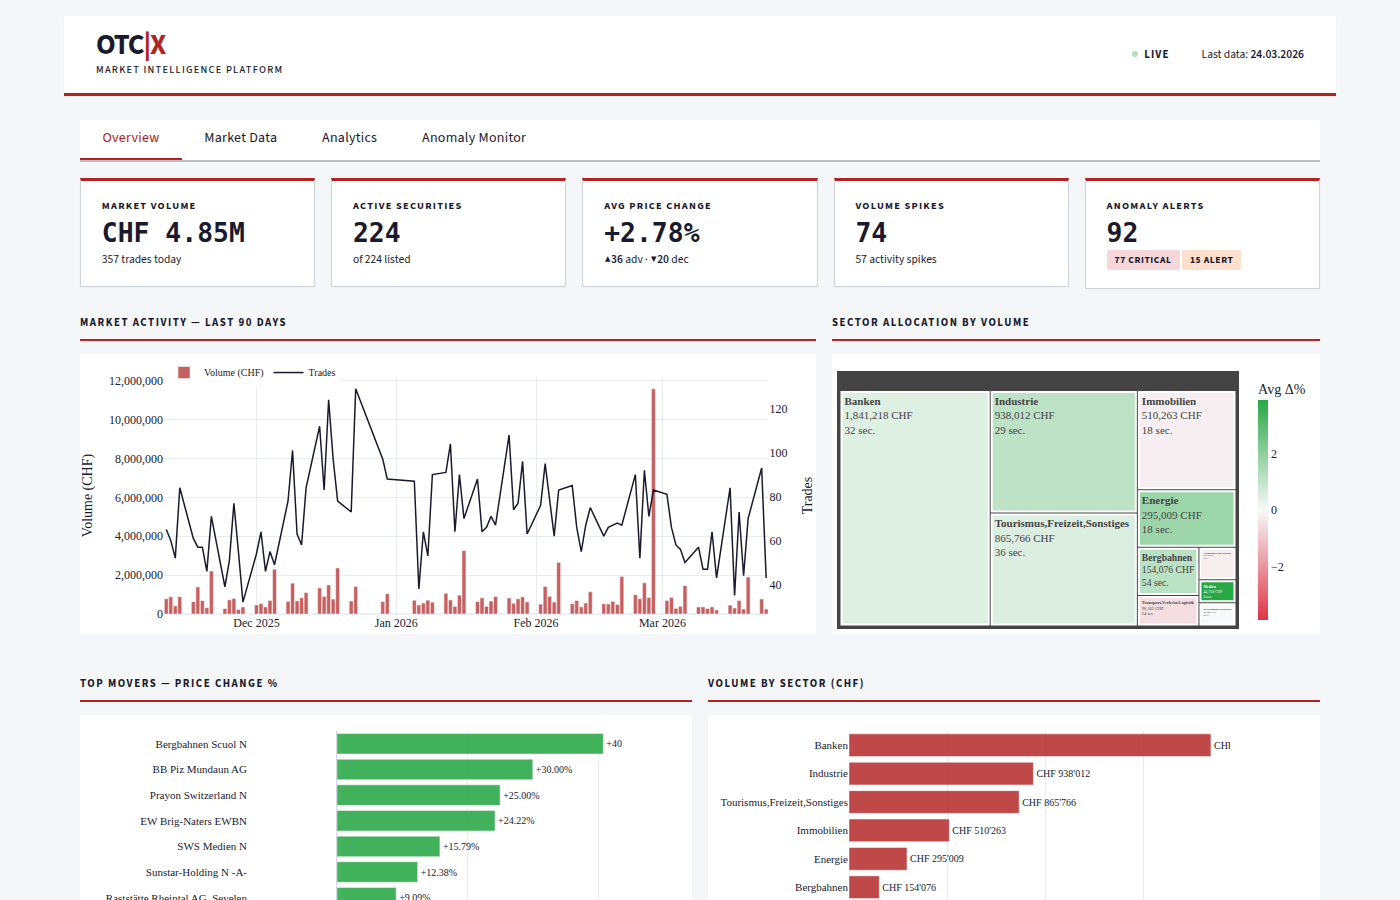
\includegraphics[width=\textwidth]{screenshots/tab-overview.png}
\caption{Overview-Tab\;---\;KPI-Karten, Sektor-Treemap und Top Movers}
\label{fig:tab-overview}
\end{figure}

\begin{figure}[H]
\centering
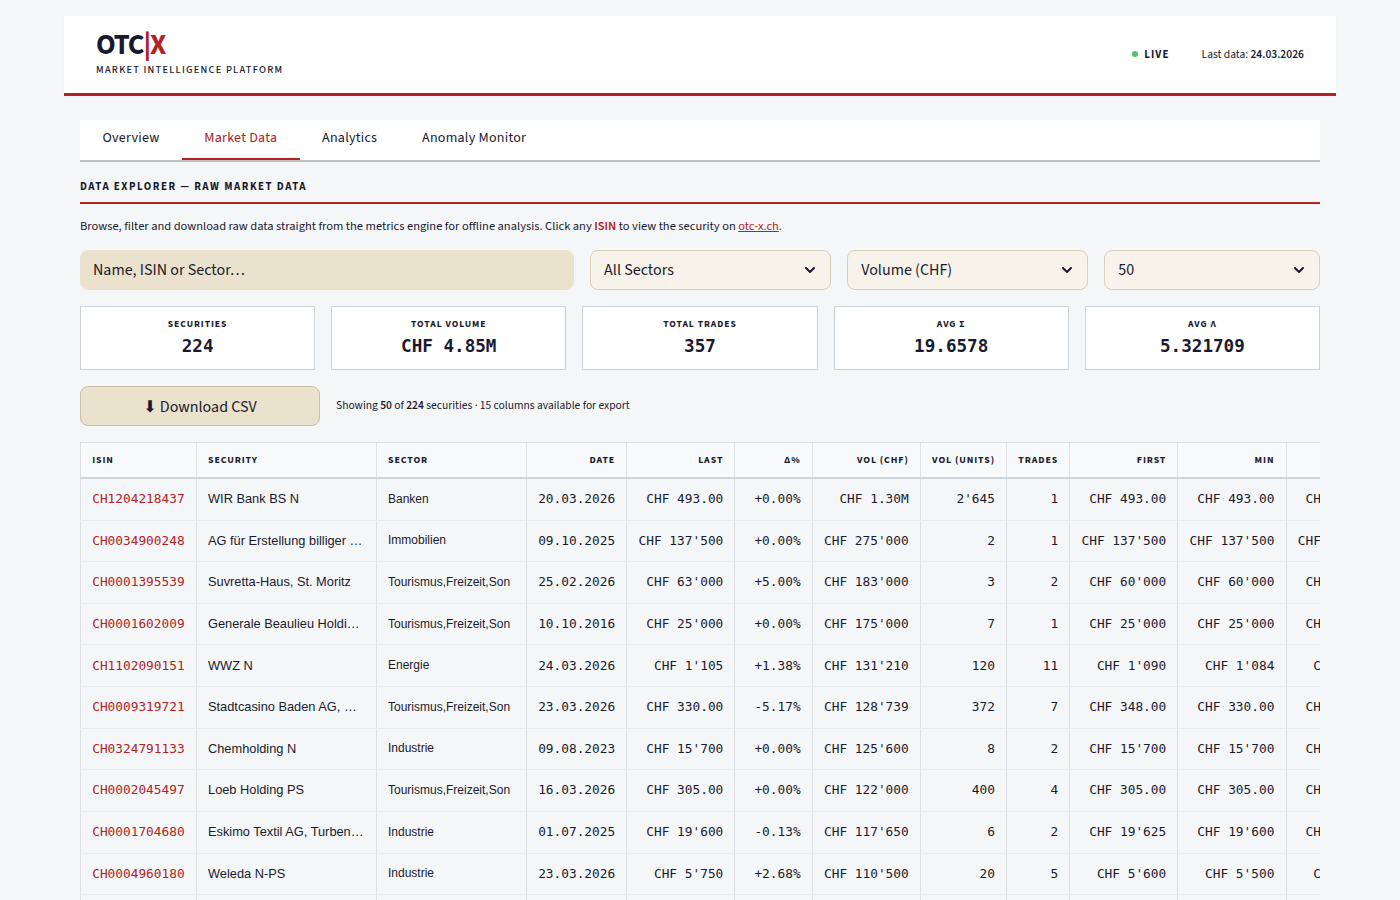
\includegraphics[width=\textwidth]{screenshots/tab-market-data.png}
\caption{Market-Data-Tab\;---\;26-Spalten-Explorer mit Security-Deep-Dive}
\label{fig:tab-market-data}
\end{figure}

\begin{figure}[H]
\centering
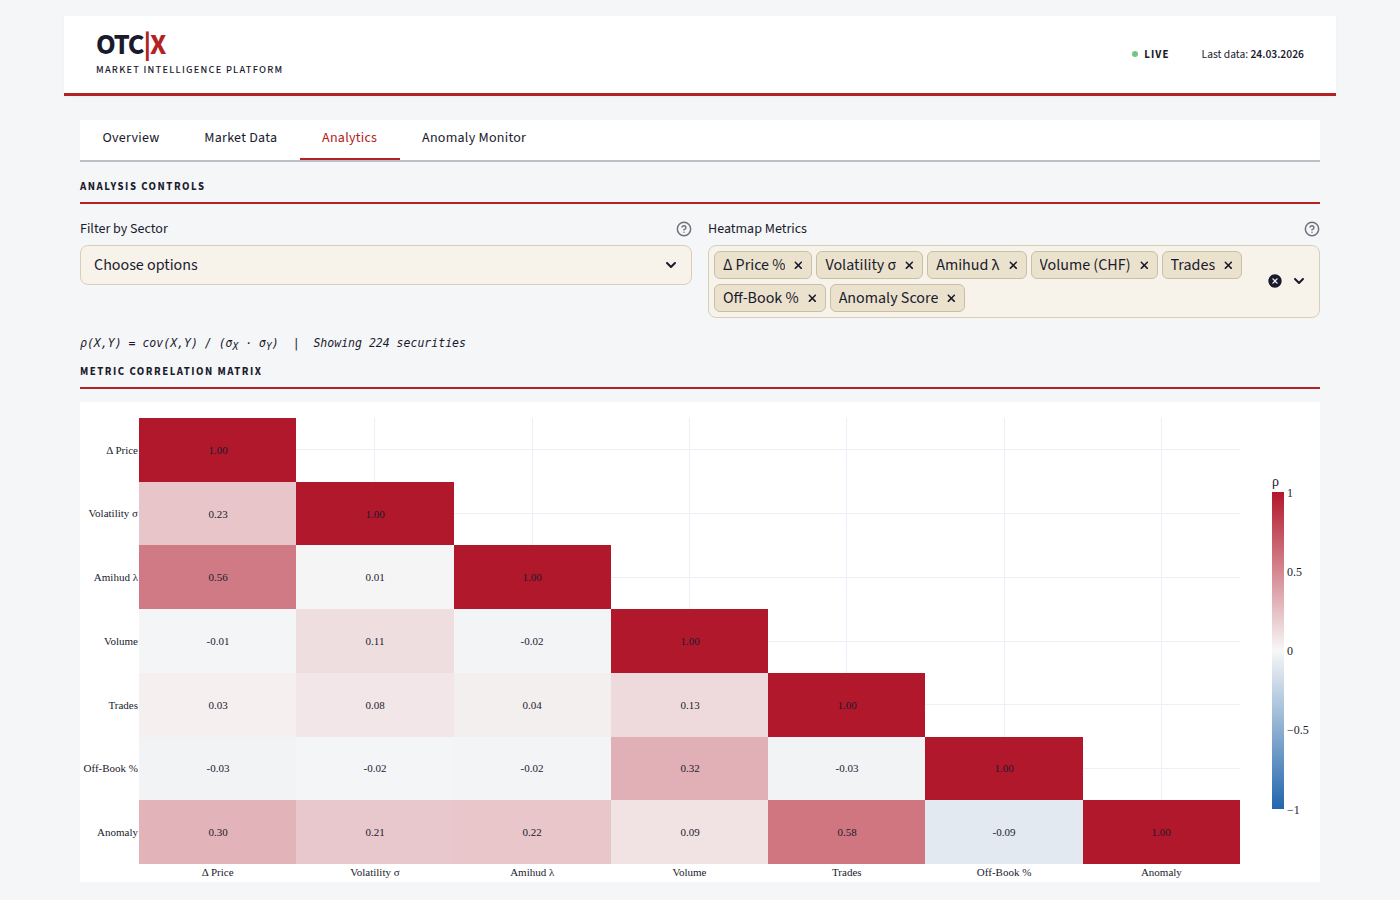
\includegraphics[width=\textwidth]{screenshots/tab-analytics.png}
\caption{Analytics-Tab\;---\;Korrelationsmatrix, Amihud-Boxplots und 3D-Explorer}
\label{fig:tab-analytics}
\end{figure}

\begin{figure}[H]
\centering
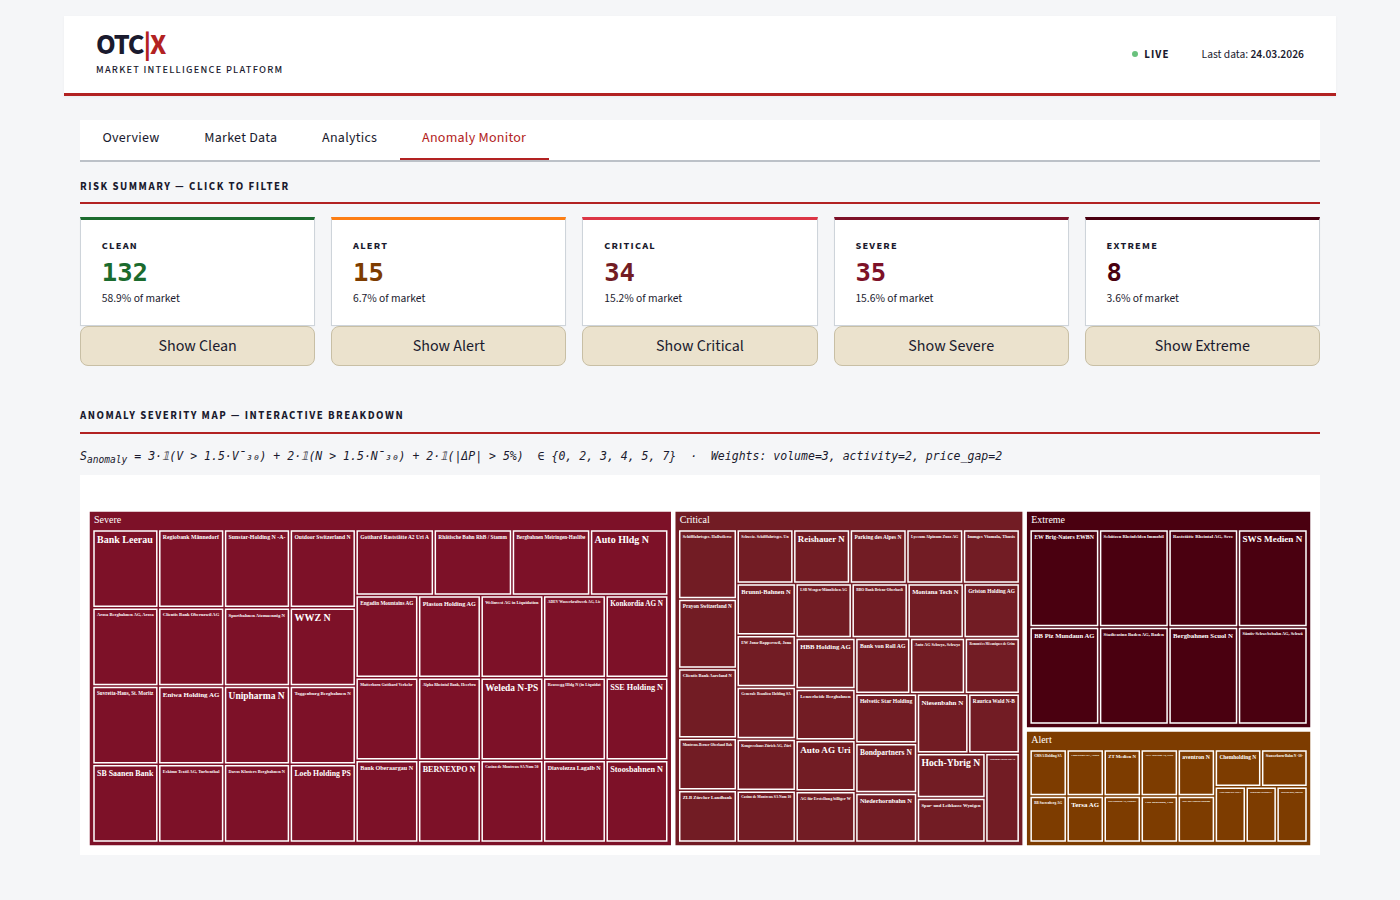
\includegraphics[width=\textwidth]{screenshots/tab-anomaly.png}
\caption{Anomaly-Monitor-Tab\;---\;Severity-Karten und Alert-Tabelle}
\label{fig:tab-anomaly}
\end{figure}


% =============================================================================
%  KAPITEL 9 --- QUALITAETSSICHERUNG UND ENGINEERING-STANDARDS
% =============================================================================
\chapter{Qualit\"atssicherung und Engineering-Standards}
\label{ch:testing}

\section{Testsuite}

Die Codebasis wird durch \textbf{118 automatisierte Tests} (pytest) in sechs Kategorien abgesichert:

\begin{table}[H]
\centering
\caption{Teststruktur nach Kategorie}
\label{tab:test-modules}
\rowcolors{2}{softgray}{white}
\begin{tabularx}{\textwidth}{>{\bfseries\sffamily}p{3.5cm} >{\centering\arraybackslash}p{1.5cm} p{2.5cm} X}
  \toprule
  \rowcolor{darknavy} \textcolor{white}{Testmodul} & \textcolor{white}{Tests} & \textcolor{white}{Kategorie} & \textcolor{white}{Abdeckung} \\
  \midrule
  test\_paths.py       & 15 & Integration        & Pfadaufl\"osung, Datei-Existenzpr\"ufung \"uber alle Module \\
  test\_backend.py     & 9  & Unit + Integration & ISIN-Berechnung (Luhn), Metriken-Engine, Pipeline-Imports \\
  test\_frontend.py    & 34 & Unit + Smoke       & Formatierungs-Utilities (CHF, \%, Badge), Config-Konsistenz, Chart-Instantiierung \\
  test\_integration.py & 24 & Integration        & End-to-End-Datenfluss, Modul-Interaktion \\
  test\_system.py      & 22 & System             & Vollst\"andige System-Level-Validierung \\
  test\_acceptance.py  & 14 & BDD/Akzeptanz      & Behaviour-Driven Tests mit pytest-bdd \\
  \bottomrule
\end{tabularx}
\end{table}

\section{Testausf\"uhrung}

\begin{lstlisting}[language=bash, caption={Testausf\"uhrung}]
python -m pytest tests/ -v
# Ergebnis: 118 Tests in ~3 Sekunden
\end{lstlisting}

S\"amtliche Tests sind so konzipiert, dass sie ohne das vollst\"andige Dataset und ohne Live-API-Zugang ausf\"uhrbar sind, was sowohl schnelles Feedback w\"ahrend der Entwicklung als auch zuverl\"assige CI-Validierung gew\"ahrleistet.

\section{Verifikationsstrategie pro Anforderung}

Jede funktionale und nicht-funktionale Anforderung ist auf mindestens eine Verifikationsmethode r\"uckf\"uhrbar:

\begin{itemize}
  \item \textbf{Automatisierte Tests}\;--- Korrektheit von Berechnungen, Imports und Formatierern
  \item \textbf{Pipeline-Receipts}\;--- Performance-Metriken, Datenprodukt-Statistiken
  \item \textbf{Manuelle Akzeptanzpr\"ufung}\;--- Dashboard-Interaktivit\"at, visuelle Korrektheit
  \item \textbf{Schema-Validierung}\;--- Parquet-Spaltentypen und -Reihenfolge
\end{itemize}

\section{Code-Konventionen}

\begin{itemize}
  \item \textbf{Type Hints:} Alle Funktionssignaturen tragen vollst\"andige Typannotationen (PEP\,484).
  \item \textbf{Docstrings:} NumPy-Style mit \code{Parameters}, \code{Returns}, \code{Raises} und \code{Notes}-Sektionen.
  \item \textbf{Pfadaufl\"osung:} Ausschliesslich via \code{Path(\_\_file\_\_).resolve().parent}-Ketten; keine hartkodierten Pfade.
  \item \textbf{Zahlenformatierung:} Schweizer Konventionen (Apostroph als Tausendertrenner, CHF-W\"ahrung).
  \item \textbf{Backend/Frontend-Separation:} Backend nutzt Polars; Frontend nutzt Pandas. Keine Vermischung.
  \item \textbf{Sicherheit:} Alle HTTP-Requests mit Timeout-Parameter; alle nutzerseitigen Daten HTML-escaped vor Markdown-Injection.
\end{itemize}

\section{CI/CD-Automatisierung}

Die GitHub-Actions-Pipeline f\"uhrt den vollst\"andigen ETL-Zyklus t\"aglich um 05:00\,UTC aus und committet die aktualisierten Datenartefakte automatisch zur\"uck ins Repository:

\begin{lstlisting}[language=bash, caption={GitHub Actions Workflow (automation\_pipeline.yml)}]
name: OTC-X Daily Pipeline
on:
  schedule:
    - cron: '0 5 * * *'
  workflow_dispatch:

permissions:
  contents: write

jobs:
  run-pipeline:
    runs-on: ubuntu-latest
    steps:
      - uses: actions/checkout@v4
      - uses: actions/setup-python@v5
        with:
          python-version: '3.10'
          cache: 'pip'
      - run: pip install -r requirements.txt
      - run: python -m backend.pipeline
      - run: |
          git config user.name 'github-actions[bot]'
          git config user.email 'github-actions[bot]@users.noreply.github.com'
          git add backend/data/ backend/logs/
          git commit -m "Automated daily OTC-X data update" || true
          git push
\end{lstlisting}


% =============================================================================
%  APPENDIX A --- OUTPUT-SCHEMA REFERENCE
% =============================================================================
\appendix

\chapter{Output-Schema Reference}
\label{app:schema}

\begin{longtable}{c >{\ttfamily}l l p{6cm}}
\caption{Vollst\"andiges Schema von \code{daily\_metrics.parquet} (26 Spalten)} \\
\toprule
\textbf{\#} & \textbf{Spalte} & \textbf{Typ} & \textbf{Beschreibung} \\
\midrule
\endfirsthead
\caption[]{(Fortsetzung)} \\
\toprule
\textbf{\#} & \textbf{Spalte} & \textbf{Typ} & \textbf{Beschreibung} \\
\midrule
\endhead
\bottomrule
\endfoot
\rowcolor{softgray}
1  & Isin                  & String   & International Securities Identification Number \\
2  & Name                  & String   & Firmenname (aus Wertpapier-Metadaten) \\
\rowcolor{softgray}
3  & Sektor                & String   & Wirtschaftssektorklassifikation \\
4  & Datum                 & Date     & Handelstag \\
\rowcolor{softgray}
5  & trades\_today          & UInt32   & Anzahl Trades an diesem Datum \\
6  & volume\_today\_units    & Float64  & Gesamtvolumen in St\"uck \\
\rowcolor{softgray}
7  & volume\_today\_chf      & Float64  & Gesamtvolumen in CHF \\
8  & price\_min             & Float64  & Intraday-Tiefstkurs \\
\rowcolor{softgray}
9  & price\_max             & Float64  & Intraday-H\"ochstkurs \\
10 & price\_first           & Float64  & Er\"offnungskurs (erster Trade des Tages) \\
\rowcolor{softgray}
11 & price\_last            & Float64  & Schlusskurs (letzter Trade des Tages) \\
12 & price\_change\_pct      & Float64  & T\"agliche Preis\"anderung (\%) \\
\rowcolor{softgray}
13 & log\_returns           & Float64  & Nat\"urlicher Logarithmus des Preisverh\"altnisses \\
14 & volatility\_daily      & Float64  & Intraday-Standardabweichung der Preise \\
\rowcolor{softgray}
15 & amihud\_daily          & Float64  & Amihud-Illiquidit\"atsratio ($\lambda$) \\
16 & spread\_log\_hl         & Float64  & Logarithmischer Hoch-Tief-Spread-Proxy \\
\rowcolor{softgray}
17 & trade\_duration\_min    & Float64  & Maximale L\"ucke zwischen Trades (Min.) \\
18 & off\_book\_pct          & Float64  & Anteil ausserb\"orslicher Trades \\
\rowcolor{softgray}
19 & trades\_30d\_median     & Float64  & 30-Handelstage-Rolling-Median der Trade-Anzahl \\
20 & volume\_30d\_median     & Float64  & 30-Handelstage-Rolling-Median des CHF-Volumens \\
\rowcolor{softgray}
21 & volatility\_30d\_median & Float64  & 30-Handelstage-Rolling-Median der Volatilit\"at \\
22 & amihud\_30d\_median     & Float64  & 30-Handelstage-Rolling-Median des Amihud $\lambda$ \\
\rowcolor{softgray}
23 & volume\_spike          & Boolean  & Flag: $V > 1{,}5 \times \tilde{V}_{30}$ \\
24 & activity\_spike        & Boolean  & Flag: $N > 1{,}5 \times \tilde{N}_{30}$ \\
\rowcolor{softgray}
25 & price\_gap             & Boolean  & Flag: $|\Delta P\%| > 5$ \\
26 & anomaly\_score         & UInt8    & Composite Anomaly Score $\in [0, 7]$ \\
\end{longtable}


% =============================================================================
%  APPENDIX B --- GLOSSAR UND ABKUERZUNGSVERZEICHNIS
% =============================================================================
\chapter{Glossar und Abk\"urzungsverzeichnis}
\label{app:glossary}

\begin{table}[H]
\centering
\rowcolors{2}{softgray}{white}
\begin{tabularx}{\textwidth}{>{\bfseries\sffamily}p{3.5cm} X}
  \toprule
  \rowcolor{darknavy} \textcolor{white}{Begriff} & \textcolor{white}{Definition} \\
  \midrule
  Amihud-Ratio ($\lambda$) & Mass f\"ur den Preisimpakt pro gehandelte Volumeneinheit; hohe Werte indizieren Illiquidit\"at \\
  API           & Application Programming Interface; Programmierschnittstelle \\
  BEKB          & Berner Kantonalbank AG \\
  CHF           & Schweizer Franken \\
  CI/CD         & Continuous Integration / Continuous Deployment \\
  ETL           & Extract, Transform, Load; Datenverarbeitungsmuster \\
  EWMA          & Exponentially Weighted Moving Average \\
  IREB          & International Requirements Engineering Board; Standardisierungsgremium \\
  ISIN          & International Securities Identification Number; 12-stelliger Code \\
  Luhn-Algorithmus & Pr\"ufzifferverfahren nach ISO 7812 zur Validierung von Identifikationsnummern \\
  MoSCoW        & Must/Should/Could/Won't; Priorisierungsmethode \\
  OTC-X         & Ausserb\"orsliche Handelsplattform der BEKB f\"ur Schweizer Titel \\
  Parquet       & Spaltenorientiertes Speicherformat f\"ur analytische Workloads (Apache Foundation) \\
  Polars        & Hochperformante DataFrame-Engine in Rust mit Python-API \\
  Rolling Median & Gleitender Median \"uber ein definiertes Zeitfenster; robust gegen\"uber Ausreissern \\
  Severity-Tier & Klassifikationsstufe (Clean bis Extreme) basierend auf dem Composite Anomaly Score \\
  SMA           & Simple Moving Average; einfacher gleitender Durchschnitt \\
  Spread Proxy  & Approximation der Geld-Brief-Spanne via logarithmisches Hoch-Tief-Verh\"altnis \\
  Streamlit     & Open-Source Python-Framework f\"ur interaktive Webapplikationen \\
  Valor         & Schweizerische Wertpapieridentifikationsnummer (6--7 Ziffern) \\
  Zstd          & Zstandard-Kompression; verlustfreier Kompressionsalgorithmus \\
  \bottomrule
\end{tabularx}
\end{table}


% =============================================================================
%  APPENDIX C --- LITERATUR UND STANDARDS
% =============================================================================
\chapter{Literatur und Standards}
\label{app:references}

\begin{enumerate}
  \item Amihud, Y. (2002). \textit{Illiquidity and stock returns: cross-section and time-series effects.} Journal of Financial Markets, 5(1), 31--56.
  \item Corwin, S.\,A. \& Schultz, P. (2012). \textit{A simple way to estimate bid-ask spreads from daily high and low prices.} The Journal of Finance, 67(2), 719--760.
  \item IREB (2023). \textit{Certified Professional for Requirements Engineering\,---\,Foundation Level Syllabus}, Version 3.1.2. International Requirements Engineering Board.
  \item ISO 6166:2021. \textit{Financial services\,---\,International securities identification number (ISIN)}. International Organization for Standardization.
  \item ISO 7812-1:2017. \textit{Identification cards\,---\,Identification of issuers\,---\,Part 1: Numbering system} (Luhn algorithm).
  \item ISO 9241-210:2019. \textit{Ergonomics of human-system interaction\,---\,Part 210: Human-centred design for interactive systems}.
  \item McKinney, W. (2017). \textit{Python for Data Analysis}, 2nd ed. O'Reilly Media.
  \item Ritchie, J. et al. (2024). \textit{Polars: Blazingly fast DataFrames in Rust and Python.} \url{https://pola.rs}
  \item Pohl, K. \& Rupp, C. (2021). \textit{Requirements Engineering Fundamentals}, 2nd ed. Rocky Nook.
\end{enumerate}


% =============================================================================
%  COLOPHON
% =============================================================================

\vfill

\begin{center}
{\color{swissred}\rule{0.4\textwidth}{1pt}}

\vspace{0.5cm}
{\small\sffamily\textcolor{darknavy}{Dieses Dokument ist Bestandteil des propriet\"aren OTC-X Projekts.}}\\
{\small\sffamily\textcolor{darknavy}{\textcopyright{} 2026 Mihael Atanasov\;\textbullet\;Alle Rechte vorbehalten.}}\\
{\small\sffamily\textcolor{darknavy}{Erstellt f\"ur die Berner Kantonalbank AG, Schwarzenburgstrasse 160, 3001 Bern.}}

\vspace{0.3cm}
{\footnotesize\sffamily\textcolor{gray}{OTC\,|\,X\;\;\textbullet\;\;Liquidity Intelligence Radar\;\;\textbullet\;\;Swiss OTC Market Intelligence}}\\[4pt]
{\footnotesize\sffamily\textcolor{gray}{Mit Pr\"azision entwickelt\;\;\textbullet\;\;f\"ur den Schweizer OTC-Markt}}\\[4pt]
{\footnotesize\sffamily\textcolor{gray}{M\"arz 2026}}

\vspace{0.5cm}
{\color{swissred}\rule{0.4\textwidth}{1pt}}
\end{center}

\end{document}
